% Options for packages loaded elsewhere
\PassOptionsToPackage{unicode}{hyperref}
\PassOptionsToPackage{hyphens}{url}
%
\documentclass[
  11pt,
  a4paper,
  oneside]{scrbook}

\usepackage{amsmath,amssymb}
\usepackage{iftex}
\ifPDFTeX
  \usepackage[T1]{fontenc}
  \usepackage[utf8]{inputenc}
  \usepackage{textcomp} % provide euro and other symbols
\else % if luatex or xetex
  \usepackage{unicode-math}
  \defaultfontfeatures{Scale=MatchLowercase}
  \defaultfontfeatures[\rmfamily]{Ligatures=TeX,Scale=1}
\fi
\usepackage{lmodern}
\ifPDFTeX\else  
    % xetex/luatex font selection
\fi
% Use upquote if available, for straight quotes in verbatim environments
\IfFileExists{upquote.sty}{\usepackage{upquote}}{}
\IfFileExists{microtype.sty}{% use microtype if available
  \usepackage[]{microtype}
  \UseMicrotypeSet[protrusion]{basicmath} % disable protrusion for tt fonts
}{}
\makeatletter
\@ifundefined{KOMAClassName}{% if non-KOMA class
  \IfFileExists{parskip.sty}{%
    \usepackage{parskip}
  }{% else
    \setlength{\parindent}{0pt}
    \setlength{\parskip}{6pt plus 2pt minus 1pt}}
}{% if KOMA class
  \KOMAoptions{parskip=half}}
\makeatother
\usepackage{xcolor}
\setlength{\emergencystretch}{3em} % prevent overfull lines
\setcounter{secnumdepth}{5}
% Make \paragraph and \subparagraph free-standing
\ifx\paragraph\undefined\else
  \let\oldparagraph\paragraph
  \renewcommand{\paragraph}[1]{\oldparagraph{#1}\mbox{}}
\fi
\ifx\subparagraph\undefined\else
  \let\oldsubparagraph\subparagraph
  \renewcommand{\subparagraph}[1]{\oldsubparagraph{#1}\mbox{}}
\fi


\providecommand{\tightlist}{%
  \setlength{\itemsep}{0pt}\setlength{\parskip}{0pt}}\usepackage{longtable,booktabs,array}
\usepackage{calc} % for calculating minipage widths
% Correct order of tables after \paragraph or \subparagraph
\usepackage{etoolbox}
\makeatletter
\patchcmd\longtable{\par}{\if@noskipsec\mbox{}\fi\par}{}{}
\makeatother
% Allow footnotes in longtable head/foot
\IfFileExists{footnotehyper.sty}{\usepackage{footnotehyper}}{\usepackage{footnote}}
\makesavenoteenv{longtable}
\usepackage{graphicx}
\makeatletter
\def\maxwidth{\ifdim\Gin@nat@width>\linewidth\linewidth\else\Gin@nat@width\fi}
\def\maxheight{\ifdim\Gin@nat@height>\textheight\textheight\else\Gin@nat@height\fi}
\makeatother
% Scale images if necessary, so that they will not overflow the page
% margins by default, and it is still possible to overwrite the defaults
% using explicit options in \includegraphics[width, height, ...]{}
\setkeys{Gin}{width=\maxwidth,height=\maxheight,keepaspectratio}
% Set default figure placement to htbp
\makeatletter
\def\fps@figure{htbp}
\makeatother
% definitions for citeproc citations
\NewDocumentCommand\citeproctext{}{}
\NewDocumentCommand\citeproc{mm}{%
  \begingroup\def\citeproctext{#2}\cite{#1}\endgroup}
\makeatletter
 % allow citations to break across lines
 \let\@cite@ofmt\@firstofone
 % avoid brackets around text for \cite:
 \def\@biblabel#1{}
 \def\@cite#1#2{{#1\if@tempswa , #2\fi}}
\makeatother
\newlength{\cslhangindent}
\setlength{\cslhangindent}{1.5em}
\newlength{\csllabelwidth}
\setlength{\csllabelwidth}{3em}
\newenvironment{CSLReferences}[2] % #1 hanging-indent, #2 entry-spacing
 {\begin{list}{}{%
  \setlength{\itemindent}{0pt}
  \setlength{\leftmargin}{0pt}
  \setlength{\parsep}{0pt}
  % turn on hanging indent if param 1 is 1
  \ifodd #1
   \setlength{\leftmargin}{\cslhangindent}
   \setlength{\itemindent}{-1\cslhangindent}
  \fi
  % set entry spacing
  \setlength{\itemsep}{#2\baselineskip}}}
 {\end{list}}
\usepackage{calc}
\newcommand{\CSLBlock}[1]{\hfill\break\parbox[t]{\linewidth}{\strut\ignorespaces#1\strut}}
\newcommand{\CSLLeftMargin}[1]{\parbox[t]{\csllabelwidth}{\strut#1\strut}}
\newcommand{\CSLRightInline}[1]{\parbox[t]{\linewidth - \csllabelwidth}{\strut#1\strut}}
\newcommand{\CSLIndent}[1]{\hspace{\cslhangindent}#1}

%----- my options----------------
\usepackage[utf8]{inputenc}
\usepackage{kotex}
\usepackage{amsmath}
\usepackage{amsfonts}
\usepackage{amssymb}

\setmainhangulfont{NanumMyeongjo}
\setsanshangulfont{NanumGothic}     % MalgunGothic
\setmonohangulfont{NanumGothic}
\setmathhangulfont{NanumGothic}

\usepackage{geometry}
 \geometry{
 a4paper,
 left=20mm,
 right=20mm,
 top=20mm,
 bottom=30mm
 }
 
\usepackage{setspace}


\newcommand{\RR}{\mathbb{R}}
\newcommand{\pardiff}[2]{\frac{\partial #1}{\partial #2 }}
\newcommand{\pardiffl}[2]{{\partial #1}/{\partial #2 }}
\newcommand{\pardiffd}[2]{\frac{\partial^2 #1}{\partial #2^t \partial #2 }}
\newcommand{\pardiffdd}[3]{\frac{\partial^2 #1}{\partial #2 \partial #3 }}
\newcommand{\norm}[1]{\left\lVert#1\right\rVert}
\newcommand{\hatmat}{\pmb X ({\pmb X}^t {\pmb X} )^{-1} {\pmb X}^t}
\newcommand{\hatmatt}[1]{\pmb X_{#1} ({\pmb X}_{#1}^t {\pmb X}_{#1})^{-1} {\pmb X}_{#1}^t}


\onehalfspacing
\makeatletter
\@ifpackageloaded{tcolorbox}{}{\usepackage[skins,breakable]{tcolorbox}}
\@ifpackageloaded{fontawesome5}{}{\usepackage{fontawesome5}}
\definecolor{quarto-callout-color}{HTML}{909090}
\definecolor{quarto-callout-note-color}{HTML}{0758E5}
\definecolor{quarto-callout-important-color}{HTML}{CC1914}
\definecolor{quarto-callout-warning-color}{HTML}{EB9113}
\definecolor{quarto-callout-tip-color}{HTML}{00A047}
\definecolor{quarto-callout-caution-color}{HTML}{FC5300}
\definecolor{quarto-callout-color-frame}{HTML}{acacac}
\definecolor{quarto-callout-note-color-frame}{HTML}{4582ec}
\definecolor{quarto-callout-important-color-frame}{HTML}{d9534f}
\definecolor{quarto-callout-warning-color-frame}{HTML}{f0ad4e}
\definecolor{quarto-callout-tip-color-frame}{HTML}{02b875}
\definecolor{quarto-callout-caution-color-frame}{HTML}{fd7e14}
\makeatother
\makeatletter
\@ifpackageloaded{bookmark}{}{\usepackage{bookmark}}
\makeatother
\makeatletter
\@ifpackageloaded{caption}{}{\usepackage{caption}}
\AtBeginDocument{%
\ifdefined\contentsname
  \renewcommand*\contentsname{목차}
\else
  \newcommand\contentsname{목차}
\fi
\ifdefined\listfigurename
  \renewcommand*\listfigurename{그림 목록}
\else
  \newcommand\listfigurename{그림 목록}
\fi
\ifdefined\listtablename
  \renewcommand*\listtablename{표 목록}
\else
  \newcommand\listtablename{표 목록}
\fi
\ifdefined\figurename
  \renewcommand*\figurename{그림}
\else
  \newcommand\figurename{그림}
\fi
\ifdefined\tablename
  \renewcommand*\tablename{표}
\else
  \newcommand\tablename{표}
\fi
}
\@ifpackageloaded{float}{}{\usepackage{float}}
\floatstyle{ruled}
\@ifundefined{c@chapter}{\newfloat{codelisting}{h}{lop}}{\newfloat{codelisting}{h}{lop}[chapter]}
\floatname{codelisting}{목록}
\newcommand*\listoflistings{\listof{codelisting}{코드 목록}}
\usepackage{amsthm}
\theoremstyle{definition}
\newtheorem{definition}{정의}[chapter]
\theoremstyle{definition}
\newtheorem{exercise}{예제}[chapter]
\theoremstyle{plain}
\newtheorem{theorem}{정리}[chapter]
\theoremstyle{remark}
\AtBeginDocument{\renewcommand*{\proofname}{증명}}
\newtheorem*{remark}{주석}
\newtheorem*{solution}{해답}
\makeatother
\makeatletter
\makeatother
\makeatletter
\@ifpackageloaded{caption}{}{\usepackage{caption}}
\@ifpackageloaded{subcaption}{}{\usepackage{subcaption}}
\makeatother
\ifLuaTeX
\usepackage[bidi=basic]{babel}
\else
\usepackage[bidi=default]{babel}
\fi
\babelprovide[main,import]{korean}
% get rid of language-specific shorthands (see #6817):
\let\LanguageShortHands\languageshorthands
\def\languageshorthands#1{}
\ifLuaTeX
  \usepackage{selnolig}  % disable illegal ligatures
\fi
\IfFileExists{bookmark.sty}{\usepackage{bookmark}}{\usepackage{hyperref}}
\IfFileExists{xurl.sty}{\usepackage{xurl}}{} % add URL line breaks if available
\urlstyle{same} % disable monospaced font for URLs
\hypersetup{
  pdftitle={빅데이터분석를 위한 수학},
  pdfauthor={이용희},
  pdflang={ko},
  hidelinks,
  pdfcreator={LaTeX via pandoc}}

\title{빅데이터분석를 위한 수학}
\author{이용희}
\date{2023-12-10}

\begin{document}
\frontmatter
\maketitle
\renewcommand*\contentsname{목차}
{
\setcounter{tocdepth}{2}
\tableofcontents
}
\mainmatter
\bookmarksetup{startatroot}

\chapter*{서론}\label{uxc11cuxb860}
\addcontentsline{toc}{chapter}{서론}

\markboth{서론}{서론}

이 온라인 연습장은 \textbf{빅데이터분석를 위한 수학}의 강의 보충 노트와
연습문제를 모아 놓은 사이트입니다.

\begin{itemize}
\item
  이 연습장은 강의에 사용된 슬라이드와 부교재 Deisenroth, Faisal, 와/과
  Ong (2020) 를 참고하였다.

  \begin{itemize}
  \tightlist
  \item
    강의에 사용된 슬라이드는 서울시립대학교 온라인 강의실에서 다운로드
    받을 수 있다.
  \item
    강의에 사용된 부교재는 \href{https://mml-book.github.io/}{교과서
    웹사이트}에서 다운로드 받을 수 있다.
  \end{itemize}
\item
  이 교재의 각 장에서는 강의에 사용된 슬라이드에서 배운 내용을 보충
  설명하고 반드시 학습해야 할 주요 주제를 설명한다.
\end{itemize}

\begin{tcolorbox}[enhanced jigsaw, colback=white, colframe=quarto-callout-note-color-frame, opacityback=0, toprule=.15mm, leftrule=.75mm, titlerule=0mm, opacitybacktitle=0.6, title=\textcolor{quarto-callout-note-color}{\faInfo}\hspace{0.5em}{노트}, colbacktitle=quarto-callout-note-color!10!white, breakable, bottomrule=.15mm, bottomtitle=1mm, toptitle=1mm, arc=.35mm, left=2mm, rightrule=.15mm, coltitle=black]

\begin{itemize}
\item
  이 연습장의 각 장(chapter)의 내용은 강의에 사용된 슬라이드 번호의
  내용과 일치합니다.
\item
  이 연습장에서 벡터와 행렬은 각각 \(\pmb x\), \(\pmb A\) 와 같이
  볼드체로 표기하며 하나의 숫자를 나타내는 변수는 보통의 서체 \(x\) 로
  표기한다.
\item
  정의, 정리, 예제 등이 끝나는 표시는 \(\blacksquare\) 로 나타낸다.
\end{itemize}

\end{tcolorbox}

\bookmarksetup{startatroot}

\chapter{강의 일정과 내용}\label{schedule}

\section{강의 진도}\label{uxac15uxc758-uxc9c4uxb3c4}

\begin{itemize}
\tightlist
\item
  1주차
\end{itemize}

\begin{longtable}[]{@{}clll@{}}
\toprule\noalign{}
슬라이드 & 주제 & 페이지 번호 & 부교재 내용 \\
\midrule\noalign{}
\endhead
\bottomrule\noalign{}
\endlastfoot
2 & 행렬의 도입 & 2-9, 13-17 & \\
3 & 행렬의 연산 & 1-3, 6-7, 9-12 & \\
\end{longtable}

\begin{itemize}
\tightlist
\item
  2주차
\end{itemize}

\begin{longtable}[]{@{}clll@{}}
\toprule\noalign{}
슬라이드 & 주제 & 페이지 번호 & 부교재 내용 \\
\midrule\noalign{}
\endhead
\bottomrule\noalign{}
\endlastfoot
4 & 역행렬과 연립방정식의 해 & 1-5 & \\
5 & 가우스소거법과 연립방정식의 해 & 1-21 & 27-32 페이지 \\
6 & 행연산 행렬과 역행렬 & & 33-34 페이지 \\
\end{longtable}

\begin{itemize}
\tightlist
\item
  3주차
\end{itemize}

\begin{longtable}[]{@{}clll@{}}
\toprule\noalign{}
슬라이드 & 주제 & 페이지 번호 & 부교재 내용 \\
\midrule\noalign{}
\endhead
\bottomrule\noalign{}
\endlastfoot
7 & 벡터공간 & 6-10 & 37-40 페이지 \\
8 & 벡터공간의 기저와 차원 & 1-15 & 40-47 페이지 \\
9 & 행렬의 계수 & 4, 7 & 47-48 페이지 \\
\end{longtable}

\begin{itemize}
\item
  4주차

  \begin{itemize}
  \tightlist
  \item
    추석연휴
  \end{itemize}
\item
  5주차
\end{itemize}

\begin{longtable}[]{@{}clll@{}}
\toprule\noalign{}
슬라이드 & 주제 & 페이지 번호 & 부교재 내용 \\
\midrule\noalign{}
\endhead
\bottomrule\noalign{}
\endlastfoot
10 & 선형사상 & 1,2,4,5,6,7 & 48-49 페이지 \\
11 & 선형사상 & & 50- 53 페이지 \\
12 & 기저변환과 변환행렬 & & \\
13 & 선형변환의 핵과 상 & 1-2 & 58-60 페이지 \\
14 & 아핀공간 & & \\
\end{longtable}

\begin{itemize}
\tightlist
\item
  6주차
\end{itemize}

\begin{longtable}[]{@{}clll@{}}
\toprule\noalign{}
슬라이드 & 주제 & 페이지 번호 & 부교재 내용 \\
\midrule\noalign{}
\endhead
\bottomrule\noalign{}
\endlastfoot
15 & 유클리드공간 위에서의 내적 & 2,3,5,6,7 & 71-78 페이지 \\
16 & 벡터공간 위에서의 내적 & 1,5,7-12 & 71-78 페이지 \\
17 & 직교기저 & 1-6 & 78-80 페이지 \\
18 & 직선으로의 정사영 & 1-5 & 81-84 페이지 \\
\end{longtable}

\bookmarksetup{startatroot}

\chapter{행렬의 도입}\label{matrix}

\section{일차연립방정식}\label{uxc77cuxcc28uxc5f0uxb9bduxbc29uxc815uxc2dd}

다음과 같이 \(n\) 개의 변수 \(x_1,x_2,\dots,x_n\) 에 대한 \(m\) 개의
일차 방정식이 있다면 이를 일차연립방정식(a system of linear equations)
이라고 한다.

\begin{equation}\phantomsection\label{eq-syseq}{
\begin{aligned}
a_{11} x_1 + a_{12} x_2 + \dots + a_{1n} x_n & = y_1 \\ 
a_{21} x_1 + a_{22} x_2 + \dots + a_{2n} x_n & = y_2 \\ 
... & \\ 
a_{m1} x_1 + a_{m2} x_2 + \dots + a_{mn} x_n & = y_m 
\end{aligned}
}\end{equation}

위의 일차연립방정식(식~\ref{eq-syseq}) 에 사용된 변수
\(x_1,x_2,\dots,x_n\) 와 계수 \(a_{ij}\), \(y_i\) 으로 좀 더 보기 좋고
효율적으로 표현하기 위하여 행렬 \(\pmb A\) 와 벡터 \(\pmb x\),
\(\pmb y\) 를 다음과 같이 표기하여

\[
\pmb A =
\begin{bmatrix}
a_{11} & a_{12} & \cdots & a_{1n} \\
a_{21} & a_{22} & \cdots & a_{2n} \\
\vdots & \vdots & \ddots & \vdots \\
a_{m1} & a_{m2} & \cdots & a_{mn}
\end{bmatrix}, 
\quad
\pmb x = 
\begin{bmatrix}
x_1 \\
x_2 \\
\vdots \\
x_n
\end{bmatrix}
,\quad
\pmb y =
\begin{bmatrix}
y_1 \\
y_2 \\
\vdots \\
y_m
\end{bmatrix}
\]

식~\ref{eq-syseq} 의 일차연립방정식을 다음과 같이 표현할 수 있다.

\begin{equation}\phantomsection\label{eq-syseq2}{
{\pmb A} {\pmb x} = {\pmb y}, \text{ 즉} \quad 
\begin{bmatrix}
a_{11} & a_{12} & \cdots & a_{1n} \\
a_{21} & a_{22} & \cdots & a_{2n} \\
\vdots & \vdots & \ddots & \vdots \\
a_{m1} & a_{m2} & \cdots & a_{mn}
\end{bmatrix}
\begin{bmatrix}
x_1 \\
x_2 \\
\vdots \\
x_n
\end{bmatrix}
=
\begin{bmatrix}
y_1 \\
y_2 \\
\vdots \\
y_m
\end{bmatrix}
}\end{equation}

식~\ref{eq-syseq2} 은 \(y_i\)의 값을 계산하는 방법이 벡터 \(\pmb x\) 의
변수 \(x_1,x_2,\dots,x_n\) 와 행렬 \(\pmb A\) 의 \(i\) 번째 행에 있는
계수들 \(a_{i1}, a_{i2}, \dots a_{in}\) 을 다음과 같은 식으로 계산한다는
의미이다. 즉 일차연립방정식(식~\ref{eq-syseq}) 을 행렬 \(\pmb A\) 와
벡터 \(\pmb x\), \(\pmb y\) 로 표현한 것이다.

\[ \sum_{i=j}^n a_{ij} x_j = y_i, \quad i=1,2,\dots,m \]

이제 위에서 일차연립방정식을 표현할 때 사용한 벡터와 행렬의 정의와 기본
연산에 대하여 알아보자.

\section{행렬과 벡터}\label{uxd589uxb82cuxacfc-uxbca1uxd130}

\subsection{행렬}\label{uxd589uxb82c}

\(m\) 개의 행과 \(n\) 개의 열을 가진, 즉 \(m \times n\) 행렬은 보통
알파벳 대문자(upper case letter)로 표현하며 다음과 같은 형태로 나타낸다.

\[
\pmb A =
\begin{bmatrix}
a_{11} & a_{12} & \cdots & a_{1n} \\
a_{21} & a_{22} & \cdots & a_{2n} \\
\vdots & \vdots & \ddots & \vdots \\
a_{m1} & a_{m2} & \cdots & a_{mn}
\end{bmatrix}
=(a_{ij})~ (i=1,2,\dots,m; j=1,2,\dots,n)
\]

행렬 \(\pmb A\) 가 \(m\) 개의 행과 \(n\) 개의 열을 가진 행렬이라면
다음과 같이 표시한다.

\[  \pmb A \in \RR^{m \times n} \]

\subsection{벡터}\label{uxbca1uxd130}

벡터(vector)는 일반적인 행렬의 하나의 행 또는 하나의 열을 나타내는
이름으로 사용된다.

\begin{itemize}
\tightlist
\item
  행렬의 각 행은 \(1 \times n\) 행렬 혹은 행벡터 (row vector)라고 한다.
\item
  행렬의 각 열은 \(m \times 1\) 행렬 혹은 열벡터 (column vector)라고
  한다.
\end{itemize}

벡터는 다음과 같이 숫자를 모아 놓은 형태에 따라서 행벡터(\(\pmb r\))와
열벡터(\(\pmb c\))로 구분할 수 있다.

\[
\pmb r = 
\begin{bmatrix}
1~ 2 ~3 ~4~
\end{bmatrix}
,\quad
\pmb c = 
\begin{bmatrix}
1 \\
2 \\
3 \\
4
\end{bmatrix}
\]

또한 벡터는 위치를 나타내는 개체 (geometric vector)로 사용할 수 있다.
위치의 개념을 더 확장하면 벡터는 \(n\) 개의 숫자(element)를 순서 있게
모아 놓은 모든 집합, 즉 유클리디안 공간(Euclidean space; \(\RR^n\)) 을
구성하는 개체로 사용할 수 있다.

\section{중요한 내용과
정의}\label{uxc911uxc694uxd55c-uxb0b4uxc6a9uxacfc-uxc815uxc758}

\begin{itemize}
\tightlist
\item
  두 행렬이 같다는 정의
\end{itemize}

\[ \pmb A = \pmb B  ~~~ \Leftrightarrow ~~~ a_{ij} =b_{ij} ~~~\forall i,j \]

\begin{itemize}
\tightlist
\item
  정방행렬(square matrix)
\item
  대각행렬(diagonal matrix)
\item
  상삼각 행렬(upper triangular matrix)과 하삼각행렬(lower triangular
  matrix)
\item
  영행렬(zero matrix)
\item
  단위행렬(identity matrix)
\item
  대칭행렬(symmetric matrix)
\item
  스칼라(scalar)
\end{itemize}

\bookmarksetup{startatroot}

\chapter{행렬의 연산}\label{matrix_compute}

\section{행렬의 덧셈과
스칼라곱}\label{uxd589uxb82cuxc758-uxb367uxc148uxacfc-uxc2a4uxce7cuxb77cuxacf1}

\subsection{덧셈}\label{uxb367uxc148}

두 행렬 \(\pmb A\) 와 \(\pmb B\) 를 더하는 규칙은 다음과 같다.

\begin{itemize}
\tightlist
\item
  두 행렬 \(\pmb A\) 와 \(\pmb B\) 는 행과 열의 갯수가 같아야 한다.
\item
  \(\pmb A + \pmb B = \pmb C\) 라고 하면, 덧셈의 결과로 만들어진 행렬
  \(\pmb C\)는 두 행렬과 같은 수의 행과 열을 가지면 각 원소는 다음과
  같다.
\end{itemize}

\[ \pmb A + \pmb B = \pmb C \quad \rightarrow \quad c_{ij} = a_{ij} + b_{ij} \]

\subsection{스칼라곱}\label{uxc2a4uxce7cuxb77cuxacf1}

임의의 실수 \(\lambda\) (스칼라)가 주어졌을 때, \(\lambda\) 와 행렬
\(\pmb A\)의 스칼라곱(scalar product) 는 행렬의 모든 원소에 \(\lambda\)
를 곱해준 행렬로 정의된다.

예를 들어 \(\lambda=2\), \(\pmb A \in \RR^{2\times 3}\) 인 경우

\[
\lambda \pmb A = 
2
\begin{bmatrix}
1 & 2 & 3 \\
-1 & 0 & 2
\end{bmatrix}
=
\begin{bmatrix}
2 & 4 & 6 \\
-2 & 0 & 4
\end{bmatrix}
\]

\section{행렬의 곱셈}\label{uxd589uxb82cuxc758-uxacf1uxc148}

먼저 두 행렬 \(\pmb A\) 와 \(\pmb B\) 의 곱셈

\[ \pmb A \times \pmb B \equiv \pmb A \pmb B \]

을 정의하려면 다음과 같은 조건이 만족되어야 한다.

\begin{itemize}
\tightlist
\item
  행렬 \(\pmb A\) 의 열의 갯수와 행렬 \(\pmb B\) 의 행의 갯수가 같아야
  한다
\end{itemize}

따라서 두 행렬의 곱셈은 순서를 바꾸면 정의 자체가 안될 수 있다.

\begin{definition}[곱셈의
정의]\protect\hypertarget{def-matrix-product}{}\label{def-matrix-product}

이제 두 행렬 \(\pmb A \in \RR^{m \times n}\) 와
\(\pmb B \in \RR^{n \times k}\)의 곱셈은 다음과 같이 정의된다.

\[ \pmb A \pmb B =  \pmb C\]

행렬 \(\pmb C\) 는 \(m\) 개의 행과 \(k\)개의 열로 구성된
행렬이며(\(\pmb C \in \RR^{m \times k}\)) 각 원소 \(c_{ij}\)는 다음과
같이 정의된다.

\[  c_{ij} = \sum_{l=1}^n a_{il} b_{lk}, \quad i=1,2,\dots,m; j=1,2,\dots,k \]

\end{definition}

먼저 간단한 예제로 다음과 같은 두 개의 행렬의 곱을 생각해 보자.

\[
\pmb A \pmb B =
\begin{bmatrix}
1 & 2 \\
3 & 4 
\end{bmatrix}
\begin{bmatrix}
0 & 1 \\
-1 & 2
\end{bmatrix}
=
\begin{bmatrix}
(1)(0) + (2)(-1) & (1)(1) + (2)(2) \\
(3)(0) + (4)(-1) & (3)(1) + (4)(2)
\end{bmatrix}
=
\begin{bmatrix}
-2 & 5 \\
-4 & 11
\end{bmatrix}
\]

곱하는 순서를 바꾸어 계산해 보자.

\[
\pmb B \pmb A =
\begin{bmatrix}
0 & 1 \\
-1 & 2
\end{bmatrix}
\begin{bmatrix}
1 & 2 \\
3 & 4 
\end{bmatrix}
=
\begin{bmatrix}
(0)(1) + (1)(3) & (0)(2) + (1)(4) \\
(-1)(1) + (2)(3) & (-1)(2) + (2)(4)
\end{bmatrix}
=
\begin{bmatrix}
3 & 4 \\
5 & 6
\end{bmatrix}
\]

위 두 결과를 보면 행렬의 곱셈에서는 교환법칙이 성립하지 않음을 알 수
있다.

이제 차원이 다른 두 행렬의 곱셈을 살펴보자.

\[
\pmb A =
\begin{bmatrix}
1 & 2 & 3\\
3 & 2 & 1
\end{bmatrix},
\quad
\pmb B =
\begin{bmatrix}
0 & 2 \\
1 & -1 \\
0 & 1
\end{bmatrix}
\]

두 행렬의 곱셈은 정의~\ref{def-matrix-product} 에 위하여 다음과 같이
계산할 수 있다.

\[
\pmb A \pmb B =
\begin{bmatrix}
1 & 2 & 3\\
3 & 2 & 1
\end{bmatrix}
\begin{bmatrix}
0 & 2 \\
1 & -1 \\
0 & 1
\end{bmatrix}
=
\begin{bmatrix}
2 & 3 \\
2 & 5
\end{bmatrix}
\]

두 행렬의 곱하는 순서를 바꾸면 차원이 전혀 다른 행렬이 얻어진다.

\[
\pmb B \pmb A =
\begin{bmatrix}
0 & 2 \\
1 & -1 \\
0 & 1
\end{bmatrix}
\begin{bmatrix}
1 & 2 & 3\\
3 & 2 & 1
\end{bmatrix}
=
\begin{bmatrix}
6 & 4 & 2 \\
-2 & 0 & 2 \\
3 & 2 & 1
\end{bmatrix}
\]

\section{중요한 내용과
정의}\label{uxc911uxc694uxd55c-uxb0b4uxc6a9uxacfc-uxc815uxc758-1}

\begin{itemize}
\item
  행렬의 전치(transpose operation): \({\pmb A}^T\)
\item
  행렬의 더하기와 스칼라곱의 성질
\item
  행렬의 곱셈은 교환법칙이 성립하지 않는다.
\end{itemize}

\begin{equation}\phantomsection\label{eq-product-not}{  \pmb A \pmb B \ne  \pmb B \pmb A}\end{equation}

\begin{tcolorbox}[enhanced jigsaw, colback=white, colframe=quarto-callout-caution-color-frame, opacityback=0, toprule=.15mm, leftrule=.75mm, titlerule=0mm, opacitybacktitle=0.6, title=\textcolor{quarto-callout-caution-color}{\faFire}\hspace{0.5em}{주의}, colbacktitle=quarto-callout-caution-color!10!white, breakable, bottomrule=.15mm, bottomtitle=1mm, toptitle=1mm, arc=.35mm, left=2mm, rightrule=.15mm, coltitle=black]

\textbf{교환법칙이 성립하지 않는다}는 의미는 식~\ref{eq-product-not} 이
언제나 성립한다는 의미는 아니다. 아래와 같이 특별한 경우 교환법칙이
성립하는 경우도 있다.

\[
\begin{bmatrix}
1 & 2 \\
1 & 3 
\end{bmatrix}
\begin{bmatrix}
1 & 0 \\
0 & 1 
\end{bmatrix}
=
\begin{bmatrix}
1 & 2 \\
1 & 3 
\end{bmatrix}
=
\begin{bmatrix}
1 & 0 \\
0 & 1 
\end{bmatrix}
\begin{bmatrix}
1 & 2 \\
1 & 3 
\end{bmatrix}
\]

\end{tcolorbox}

\begin{itemize}
\tightlist
\item
  행렬의 곱셈은 결합법칙과 배분법칙은 성립한다.
\end{itemize}

\[ (\pmb A \pmb B) \pmb C = \pmb A (\pmb B \pmb C) \]

\[ (\pmb A + \pmb B) \pmb C = \pmb A \pmb C +  \pmb B \pmb C \]

\bookmarksetup{startatroot}

\chapter{행렬과 연립방정식의 해}\label{matrix_inverse}

\section{역행렬의 정의}\label{uxc5eduxd589uxb82cuxc758-uxc815uxc758}

정방행렬 \(\pmb A \in \RR^{n \times n}\)의 역행렬(inverse metrix)이
존재하면 \(\pmb A^{-1}\)로 표시하며 다음을 만족하는 행렬이다.

\[ \pmb A \pmb A^{-1} = \pmb A^{-1} \pmb A= \pmb I \]

\begin{itemize}
\item
  역행렬은 유일하다.
\item
  예를 들어 2차원 정방행렬의 역행렬은 다음과 같이 계산할 수 있다.
\end{itemize}

\begin{equation}\phantomsection\label{eq-inverse-22}{
\pmb A =
\begin{bmatrix}
a & b \\
c & d 
\end{bmatrix}, ad-bc \ne 0
\rightarrow
{\pmb A}^{-1} = \frac{1}{ad-bc}
\begin{bmatrix}
d & -b \\
-c & a 
\end{bmatrix}
}\end{equation}

위의 2차원 정방행렬의 역행렬에서 만약 \(ad-bc =0\) 이면 역행렬이
존재하지 않는다. 일반적으로 모든 정방행렬의 역행렬이 존재하는 것은
아니다.

\section{중요한 내용과
정의}\label{uxc911uxc694uxd55c-uxb0b4uxc6a9uxacfc-uxc815uxc758-2}

\begin{itemize}
\tightlist
\item
  역행렬의 성질
\end{itemize}

\[ (\pmb A \pmb B)^{-1} = {\pmb B}^{-1} {\pmb A}^{-1} \]

\[ (\pmb A^T)^{-1} = (\pmb A^{-1})^{T} \]

\begin{itemize}
\item
  연립방정식의 해

  \(n\)개의 \(n\) 변수 일차연립방정식 \(\pmb A \pmb x = \pmb y\)가
  주어졌다고 하자. 여기서 \(\pmb A\)는 \(n \times n\) 정방행렬이다. 만약
  \(\pmb A^{-1}\)가 존재하면

  \[ \pmb x = \pmb A^{-1} \pmb y \]
\end{itemize}

\bookmarksetup{startatroot}

\chapter{가우스소거법과 연립방정식의 해}\label{matrix_equation}

\begin{tcolorbox}[enhanced jigsaw, colback=white, colframe=quarto-callout-important-color-frame, opacityback=0, toprule=.15mm, leftrule=.75mm, titlerule=0mm, opacitybacktitle=0.6, title=\textcolor{quarto-callout-important-color}{\faExclamation}\hspace{0.5em}{중요}, colbacktitle=quarto-callout-important-color!10!white, breakable, bottomrule=.15mm, bottomtitle=1mm, toptitle=1mm, arc=.35mm, left=2mm, rightrule=.15mm, coltitle=black]

\begin{itemize}
\tightlist
\item
  슬라이드의 1-7페이지를 반드시 먼저 학습하세요
\item
  부교재 Deisenroth, Faisal, 와/과 Ong (2020) 의 다음 절을 반드시
  학습하세요

  \begin{itemize}
  \tightlist
  \item
    2.3.1 Particular and General Solution
  \item
    2.3.2 Elementary Transformations
  \item
    2.3.3 The Minus-1 Trick
  \end{itemize}
\end{itemize}

\end{tcolorbox}

\section{행렬의
기본연산}\label{uxd589uxb82cuxc758-uxae30uxbcf8uxc5f0uxc0b0}

\subsection{일차연립방정식의
기본연산}\label{uxc77cuxcc28uxc5f0uxb9bduxbc29uxc815uxc2dduxc758-uxae30uxbcf8uxc5f0uxc0b0}

기본연산은 일차연립방정식의 해집합을 변화시키지 않으면서 방정식을
변화시켜 해집합을 구하는 다음의 세 가지 연산을 말한다.

\begin{enumerate}
\def\labelenumi{\arabic{enumi}.}
\tightlist
\item
  한개의 방정식의 양변에 0이 아닌 상수를 곱하기
\item
  한개의 방정식의 양변에 0이 아닌 상수를 곱한 것을 다른방정식의 양변에
  각각 더하기\\
\item
  방정식의 위치를 바꾸기
\end{enumerate}

\subsection{행렬의 기본
행연산}\label{uxd589uxb82cuxc758-uxae30uxbcf8-uxd589uxc5f0uxc0b0}

기본 행연산(elementary row operation)은 기본연산을 행렬의 행에 시행하는
것을 말한다.

\begin{enumerate}
\def\labelenumi{\arabic{enumi}.}
\tightlist
\item
  한 행에 0이 아닌 상수를 곱하기
\item
  한 행에 0이 아닌 상수를 곱한 결과를 다른 행 에더하기
\item
  두 행의 위치를 교환하기
\end{enumerate}

\section{행렬과 벡터의 곱}\label{sec-intro-product}

\(m \times n\) 인 행렬 \(\pmb A\) 와 \(n\)-차원 벡터 \(\pmb x\)를 곱하는
과정을 다음과 같이 두 개의 서로 다른 형태로 나타낼 수 있다.

\begin{enumerate}
\def\labelenumi{\arabic{enumi}.}
\tightlist
\item
  \textbf{행렬 계산법의 이용}
\end{enumerate}

먼저 행렬과 벡터의 곱셈은 행렬 계산법의 이용하여 나타낼 수 있다.

\[
{\pmb A} {\pmb x}  = 
\begin{bmatrix}
a_{11} & a_{12} & \dots & a_{1n} \\
a_{21} & a_{22} & \dots & a_{2n} \\
\vdots & \vdots &    & \dots \\
a_{m1} & a_{m2} & \dots & a_{mn} 
\end{bmatrix}
\begin{bmatrix}
x_1 \\
x_2 \\
\vdots \\
x_n 
\end{bmatrix} 
=
\begin{bmatrix}
\sum_{l=1}^n a_{1l} x_l \\
\sum_{l=1}^n a_{2l} x_l \\
\vdots \\
\sum_{l=1}^n a_{ml} x_l
\end{bmatrix} \\
\]

\begin{enumerate}
\def\labelenumi{\arabic{enumi}.}
\setcounter{enumi}{1}
\tightlist
\item
  \textbf{열벡터의 선형조합}
\end{enumerate}

이제 행렬과 벡터의 곱셈을 행렬 \(\pmb A\)을 구성하는 열벡터들의
선형조합(linear combination)으로 나타낼 수 있다.

\[
{\pmb A} {\pmb x} = 
x_1
\begin{bmatrix}
a_{11} \\
a_{21} \\
\vdots \\
a_{m1} 
\end{bmatrix} 
+ 
x_2 
\begin{bmatrix}
a_{12} \\
a_{22} \\
\vdots \\
a_{m2} 
\end{bmatrix} 
+ \cdots + 
x_n 
\begin{bmatrix}
a_{1n} \\
a_{2n} \\
\vdots \\
a_{mn} 
\end{bmatrix}
=
x_1 {\pmb a}_1 + x_2 {\pmb a}_2 + \cdots + x_n {\pmb a}_n 
\]

위의 식에서 벡터 \(\pmb a_j\) 는 행렬 \(\pmb A\) 의 \(j\) 번째
열벡터이다.

\begin{exercise}[]\protect\hypertarget{exr-mat-vec-product}{}\label{exr-mat-vec-product}

먼저 간단한 예제로 다음과 같은 행렬과 벡터의 곱셈을 생각해 보자.

\[
\pmb A =
\begin{bmatrix}
1 & 2 \\
1 & -1 
\end{bmatrix},
\quad
\pmb x =
\begin{bmatrix}
1 \\
-1
\end{bmatrix}
\]

행렬과 벡터의 곱셈은 앞에서 배운 행렬의 곱셈 방법으로 다음과 같이 나타낼
수 있다.

\[
\pmb A \pmb x =
\begin{bmatrix}
1 & 2 \\
1 & -1 
\end{bmatrix}
\begin{bmatrix}
1 \\
-1
\end{bmatrix}
=
\begin{bmatrix}
(1)(1) + (2)(-1)  \\
(1)(1) + (-1)(-1) 
\end{bmatrix}
=
\begin{bmatrix}
-1 \\
2
\end{bmatrix}
\]

이제 행렬과 벡터의 곱셈을 행렬 \(\pmb A\) 의 열들의 선형 조합으로 표시할
수 있다는 것도 알아두자.

\[
\pmb A \pmb x =
\begin{bmatrix}
1 & 2 \\
1 & -1 
\end{bmatrix}
\begin{bmatrix}
1 \\
-1
\end{bmatrix}
=(1)
\begin{bmatrix}
1 \\
1
\end{bmatrix}
+ (-1)
\begin{bmatrix}
2 \\
-1
\end{bmatrix}
=
\begin{bmatrix}
-1 \\
2
\end{bmatrix}
\]

행렬과 벡터의 곱셈을을 \textbf{앞 행렬의 열}과 \textbf{뒷 벡터의 원소}의
선형조합으로 나타낼 수 있다는 사실은 다양한 주제에서 유용하게 사용된다.

\(\blacksquare\)

\end{exercise}

\section{방정식의 근이 무한개인
경우}\label{uxbc29uxc815uxc2dduxc758-uxadfcuxc774-uxbb34uxd55cuxac1cuxc778-uxacbduxc6b0}

교재 슬라이드 4번의 5-7 페이지에는 변수가 3개이고 방정식의 개수가 2개인
경우에 \begin{equation}\phantomsection\label{eq-exam-eq-1}{
\begin{cases}
x_1 - 2 x_2 + 2 x_3 = 6 \\
x_2 -x_3 =2 
\end{cases}
~~\leftrightarrow~~
\pmb A \pmb x = \pmb y
~~\leftrightarrow~~
\begin{bmatrix}
1 & -2 & 2 \\
0 & 1  & -1 
\end{bmatrix}
\begin{bmatrix}
x_1 \\
x_2 \\
x_3 \end{bmatrix}
=
\begin{bmatrix}
6 \\
2
\end{bmatrix}
}\end{equation}

아래와 같이 첨가행렬(augmented matrix)을 만들고 기본 행연산을 적용하여
일반해를 구하는 예제가 있다.

\begin{equation}\phantomsection\label{eq-exam-eq-1-aug}{
\left[\begin{array}{ccc|c}
1 & -2 & 2 & 6\\
0 & 1  & -1 & 2
\end{array}\right]
}\end{equation}

위의 식~\ref{eq-exam-eq-1-aug} 에서 첨가행렬의 왼쪽 부분이 행사다리꼴
행렬(row echelon form)임을 유의하자. 식~\ref{eq-exam-eq-1-aug} 의 두
번째 행에 2를 곱해서 첫번 째 행에 더하면 다음과 같이 기약행사다리꼴
행렬(reduced row echelon form)이 된다.

\begin{equation}\phantomsection\label{eq-exam-eq-1-aug2}{
\left[\begin{array}{ccc|c}
1 & 0 & 0 & 10\\
0 & 1  & -1 & 2
\end{array}\right]
}\end{equation}

이제 방정식을 푸는 3가지 방법에 대하여 알아보자.

\textbf{(1) 매개변수와 가우스소거법를 이용하는 법}

슬라이드에 나오는 방법처럼 식~\ref{eq-exam-eq-1-aug2} 에
매개변수(\(x_3=t\))를 사용하기 위하여 첨가행렬의 마지막 행에
\((0,0,1,t)\)를 추가한 후 첨가행렬의 왼쪽을 항등행렬로 바꾸는 행연산을
적용하면(가우스 소거법) 다음과 같은 결과를 얻고

\[
\
\left[\begin{array}{ccc|c}
1 & 0 & 0 & 10\\
0 & 1  & 0 & t+ 2 \\
0 & 0 & 1 & t
\end{array}\right]
\] 해집합은 다음과 같이 주어진다.

\begin{equation}\phantomsection\label{eq-exam-eq-1-sol}{
\begin{bmatrix}
x_1 \\
x_2 \\
x_3 
\end{bmatrix}
= 
\begin{bmatrix}
10 \\
t+2 \\
t 
\end{bmatrix}
=
t
\begin{bmatrix}
0 \\
1 \\
1 
\end{bmatrix}
+ 
\begin{bmatrix}
10 \\
2 \\
0 
\end{bmatrix}, \quad t \in \RR
}\end{equation}

\textbf{(2) 특수해와 선형조합을 이용}

다시 식~\ref{eq-exam-eq-1-aug2} 에서 제시된 방정식을 열벡터의 선형조합의
형태로 아래와 같이 써보자

\begin{equation}\phantomsection\label{eq-exam-eq-linear}{
\pmb A \pmb x = \pmb y
~~\leftrightarrow~~
x_1
\begin{bmatrix}
1  \\
0  
\end{bmatrix}
+
x_2
\begin{bmatrix}
 0  \\
 1   
\end{bmatrix}
+ x_3
\begin{bmatrix}
 0 \\
-1 
\end{bmatrix}
=
\begin{bmatrix}
10 \\
2
\end{bmatrix}
}\end{equation}

이제 위의 식에서 \(x_3=0\) 으로 놓으면 다음과 같이 \(x_1\) 과 \(x_2\) 만
포함된 간단한 방정식이 나타나며 이를 만족하는 특수해(particular
solution) \(\pmb x^*\) 를 다음과 같이 구할 수 있다.

\begin{equation}\phantomsection\label{eq-exam-eq-1-sol-2}{
x_3=0,~~
x_1
\begin{bmatrix}
1  \\
0  
\end{bmatrix}
+
x_2
\begin{bmatrix}
 0  \\
 1   
\end{bmatrix}
=
\begin{bmatrix}
10 \\
2
\end{bmatrix}
~ \rightarrow~~~
\pmb x^* =
\begin{bmatrix}
x_1 \\
x_2 \\
x_3 \end{bmatrix}
=
\begin{bmatrix}
10 \\
2 \\
0 \end{bmatrix}
}\end{equation}

위의 식~\ref{eq-exam-eq-1-sol-2} 에서 구한 특수해 \(\pmb x^*\) 는
식~\ref{eq-exam-eq-1-sol} 에서 주어진 해집합에서 나타난 마지막 벡터이다.

이제 식~\ref{eq-exam-eq-1} 에 주어진 방정식은 특별한 해 \(\pmb x^*\) 만
만족하는 것이 아니므로 일반해(general solution)을 구해야 한다. 일반해를
구하는 방법은 다음과 같이 행렬 \(\pmb A\)의 열들의 선형 조합이 영벡터가
되는 \(\pmb x^{**}\)를 찾는 것이다.

\begin{equation}\phantomsection\label{eq-exam-eq-1-sol-3}{
\pmb A \pmb x^{**} = \pmb 0
\quad \leftrightarrow \quad 
x_1
\begin{bmatrix}
1  \\
0  
\end{bmatrix}
+
x_2
\begin{bmatrix}
 0  \\
 1   
\end{bmatrix}
+ x_3
\begin{bmatrix}
 0 \\
-1 
\end{bmatrix}
=
\begin{bmatrix}
0 \\
0
\end{bmatrix}
}\end{equation}

식~\ref{eq-exam-eq-1-sol-3} 를 만족하는 해는 유일하지 않다. 하지만 행렬
\(\pmb A\)의 두 번째 열과 세 번째 열의 부호가 반대인 점을 이용하면
다음과 같은 식을 얻을 수 있다.

\[
(0)
\begin{bmatrix}
1  \\
0  
\end{bmatrix}
+
(1)
\begin{bmatrix}
 0  \\
 1   
\end{bmatrix}
+ (1)
\begin{bmatrix}
 0 \\
-1 
\end{bmatrix}
=
\begin{bmatrix}
0 \\
0
\end{bmatrix}
\] 따라서 식~\ref{eq-exam-eq-1-sol-3} 를 만족하는 해 \(\pmb x^{**}\) 는
쉽게 찾을 수 있다.

\[ \pmb x^{**} =
\begin{bmatrix}
0 \\
1 \\
1 
\end{bmatrix}
\]

이제 \(\pmb A \pmb x^{*} = \pmb y\) 를 만족하는 특수해 \(\pmb x^{*}\) 와
\(\pmb A \pmb x^{**} = \pmb 0\) 를 만족하는 \(\pmb x^{**}\) 를 이용하여
일반해를 구해보자. 임의의 실수 \(t\) 에 대하여 다음과 같은 식이
만족한다.

\[ \pmb A (\pmb x^* + t \pmb x^{**})  =
\pmb A \pmb x^* + t \pmb A \pmb x^{**}
= \pmb y + t \pmb 0 = \pmb y \quad  t \in \RR\]

위의 식에 의하여 이제 일반해를 구하면 다음과 같이 나타나며 이는
매개변수를 이용하여 얻은 해(식~\ref{eq-exam-eq-1-sol})와 동일하게
나타난다.

\[
\begin{bmatrix}
x_1 \\
x_2 \\
x_3 
\end{bmatrix}
= 
\pmb x^* + t \pmb x^{**}
=
\begin{bmatrix}
10 \\
2 \\
0 
\end{bmatrix}+
t
\begin{bmatrix}
0 \\
1 \\
1 
\end{bmatrix},
 \quad t \in \RR
\]

\textbf{(3) (-1)-추가법}

이제 마지막 방법은 부교재 2.3.3 절(32 페이지)에 나온 (-1)-추가법(Minus-1
Trick)에 대하여 배워보자.

식~\ref{eq-exam-eq-1-aug2} 는 기약행사다리꼴 행렬로서 첫 번째 행과 두
번째 행이 피봇을 포함한 행이다. 이제 기약행사다리꼴 행렬에 대각원소
위치에 피봇이 없는 행에 대각원소가 -1 인 행을 추가하여 정방행렬로 만들어
보자. 식~\ref{eq-exam-eq-1-aug2} 에서 3행에 피봇이 없으므로 대각원소가
-1 이고 나머지가 0인 행을 3행에 다음과 같이 추가한다.

\begin{equation}\phantomsection\label{eq-exam-eq-1-minus1}{
\left[\begin{array}{ccc|c}
1 & 0 & 0 & 10\\
0 & 1  & -1 & 2 \\
\color{red}{0} &  \color{red}{0} & \color{red}{-1} & \color{red}{0} 
\end{array}\right]
}\end{equation}

이제 식~\ref{eq-exam-eq-1-minus1} 에서 가장 오른 쪽에 있는 열이 특수해가
되며 대각원소가 -1 은 열벡터가 \(\pmb A \pmb x = \pmb 0\) 을 만족하는
해가 된다.

따라서 방정식의 일반해를 다음과 같이 쓸수 있다.

\[
\begin{bmatrix}
x_1 \\
x_2 \\
x_3 
\end{bmatrix}
=
\begin{bmatrix}
10 \\
2 \\
0 
\end{bmatrix}+
t^*
\begin{bmatrix}
0 \\
-1 \\
-1 
\end{bmatrix}
=
\begin{bmatrix}
10 \\
2 \\
0 
\end{bmatrix}+
t
\begin{bmatrix}
0 \\
1 \\
1 
\end{bmatrix},
 \quad t=-t^*, ~~ t \in \RR
\]

\section{영공간과
일반해}\label{uxc601uxacf5uxac04uxacfc-uxc77cuxbc18uxd574}

식~\ref{eq-exam-eq-1-sol-3} 에 나타난 것과 같이 주어진 행렬 \(\pmb A\)
의 열들의 선형조합을 영벡터로 만드는 해의 집합을 영공간(Null space)라고
한다.

\begin{definition}[]\protect\hypertarget{def-nullspace}{}\label{def-nullspace}

일차연립방정식(또는 행렬 방정식) \(\pmb A \pmb x = \pmb 0\) 의 해집합을
\(\pmb A\)의 영공간이라고 하고 \(N (\pmb A)\)라고 표시한다. 즉,

\[ N( \pmb A)=\{ \pmb x: \pmb A \pmb x= \pmb 0 \}\]

\end{definition}

위에서 방정식의 해를 찾을 때 특수한 해를 먼저 찾고 일반해를 만드는
작업은 영공간을 찾는 작업과 동일하다.

\section{중요한 내용과
정의}\label{uxc911uxc694uxd55c-uxb0b4uxc6a9uxacfc-uxc815uxc758-3}

\begin{itemize}
\tightlist
\item
  행사다리꼴 행렬(row echelon form)의 정의
\item
  피벗(pivot 혹은 leading entry)의 정의
\item
  기약행사다리꼴(reduced row echelon form)의 정의
\item
  가우스 소거법의 절차

  \begin{itemize}
  \tightlist
  \item
    기본변수(basic variable)와 자유변수(free variable)
  \item
    매개변수의 이용
  \end{itemize}
\item
  연립일차방정식이 유일한 해를 가질 조건
\item
  정방행렬의 역행령이 존재하면 영공간은 영벡터와 같다.
\end{itemize}

\bookmarksetup{startatroot}

\chapter{행연산 행렬과 역행렬}\label{matrix_inverse2}

\begin{tcolorbox}[enhanced jigsaw, colback=white, colframe=quarto-callout-important-color-frame, opacityback=0, toprule=.15mm, leftrule=.75mm, titlerule=0mm, opacitybacktitle=0.6, title=\textcolor{quarto-callout-important-color}{\faExclamation}\hspace{0.5em}{중요}, colbacktitle=quarto-callout-important-color!10!white, breakable, bottomrule=.15mm, bottomtitle=1mm, toptitle=1mm, arc=.35mm, left=2mm, rightrule=.15mm, coltitle=black]

강의자료 슬라이드 6번의 기본행렬은 강의 범위에 포함되지 않습니다.

단, 첨가행렬과 행연산을 이용하여 역행렬을 구하는 방법은 반드시 알아야
합니다.

이 연습장에 포함된 예제와 부교재 33-34 페이지 Calculating the Inverse 의
Example 2.9 를 공부하세요.

\end{tcolorbox}

\section{역행렬의 공식}\label{uxc5eduxd589uxb82cuxc758-uxacf5uxc2dd}

먼저 \(2 \times 2\) 행렬의 역행렬을 구하는 공식을 이용해 보자. 다음과
같이 \(2 \times 2\) 행렬 \(\pmb A\) 가 주어졌을 때

\[
\pmb  A =
\begin{bmatrix}
1 & 2 \\
3 & 4
\end{bmatrix}
\]

식~\ref{eq-inverse-22} 를 사용하면 다음과 같이 \(2 \times 2\) 행렬의
역행렬을 구할 수 있다.

\[ \pmb A^{-1} = \frac{1}{(1)(4)-(2)(3) }
\begin{bmatrix}
4 & -2 \\
-3 & 1
\end{bmatrix}
=
\begin{bmatrix}
-2 & 1 \\
3/2 & -1/2
\end{bmatrix}
\]

\section{행연산과
역행렬}\label{uxd589uxc5f0uxc0b0uxacfc-uxc5eduxd589uxb82c}

아래에 주어진 두 예제에서 행연산을 이용하여 역행렬을 구해보자.

\begin{exercise}[\(2 \times 2\) 행렬의
역행렬]\protect\hypertarget{exr-inverse1}{}\label{exr-inverse1}

정방행렬의 역행렬을 구하는 다른 방법 중의 하나는 항등행렬 \(\pmb I\) 와
같이 첨가행렬을 만들고 행연산을 적용하는 것이다. 이제 행연산을 이용하여
\(\pmb A\) 의 역행렬을 구하는 방법을 연습해 보자

이제 \(\pmb A\) 과 이차원 항등행렬 \(\pmb I\) 을 붙여서 만든 첨가행렬은
다음과 같다.

\[
[ ~\pmb A ~|~ \pmb I ~]=
\left[\begin{array}{cc|cc}
1 & 2 & 1 & 0\\
3 & 4  & 0 & 1
\end{array}\right]
\]

이제 위의 첨가행렬에서 행연산을 이용하여 행렬 \(\pmb A\) 부분을
항등행렬로 만들어 보자.

\[
\begin{aligned}
& 
\left[\begin{array}{cc|cc}
1 & 2 &  1 & 0\\
3 & 4 & 0 & 1 
\end{array}\right]  
\begin{array}{c}
 \\
 (-3)(\text{1st row}) + (\text{2nd row}) 
\end{array} \\
& \\
 \rightarrow &
\left[\begin{array}{cc|cc}
1 & 2  & 1 & 0\\
0 & -2 & -3 & 1 
\end{array}\right]  
\begin{array}{c}
(1)(\text{2nd row}) + (\text{1st row}) 
\\
\end{array} \\
& \\
 \rightarrow &
\left[\begin{array}{cc|cc}
1 & 0  & -2 & 1\\
0 & -2 & -3 & 1 
\end{array}\right]  
\begin{array}{c}
\\
(-1/2) (\text{2nd row}) 
\end{array} \\
& \\
 \rightarrow & 
\left[\begin{array}{cc|cc}
1 & 0  & -2 & 1\\
0 & 1 & 3/2 &-1/2 
\end{array}\right] 
\end{aligned}
\]

이렇게 첨가행렬에서 행렬 \(\pmb A\) 부분을 행연산을 이용하여 항등행렬로
만들어 주면 오른쪽의 항등행렬이 \(\pmb A^{-1}\)로 나타난다.

\(\blacksquare\)

\end{exercise}

\begin{exercise}[\(4 \times 4\) 행렬의
역행렬]\protect\hypertarget{exr-inverse2}{}\label{exr-inverse2}

\[ \pmb A =
\begin{bmatrix}
1 & 0 & 1 & 0 \\
0 & 1 & 1 & 0 \\
1 & 1 & 0 & 1 \\
1 & 1 & 1 & 0
\end{bmatrix}
\]

첨가행렬에서 행연산을 이용하여 행렬 \(\pmb A\) 부분을 항등행렬로 만들어
보자.

\[
\begin{aligned}
& \left[\begin{array}{cccc|cccc}
1 & 0 & 1 & 0 & 1 & 0 & 0 & 0\\
0 & 1 & 1 & 0 & 0 & 1 & 0 & 0\\
1 & 1 & 0 & 1 & 0 & 0 & 1 & 0\\
1 & 1 & 1 & 0 & 0 & 0 & 0 & 1
\end{array}\right]  
\begin{array}{c}
 \\
 \\
(-1)(\text{1st row}) + (\text{3nd row}) \\
(-1)(\text{1st row}) + (\text{4th row}) 
\end{array}  \\
& \\
\rightarrow & 
 \left[\begin{array}{cccc|cccc}
1 & 0 & 1 & 0 & 1 & 0 & 0 & 0\\
0 & 1 & 1 & 0 & 0 & 1 & 0 & 0\\
0 & 1 & -1 & 1 & -1 & 0 & 1 & 0\\
0 & 1 & 0  & 0 & -1 & 0 & 0 & 1
\end{array}\right]  
\begin{array}{c}
 \\
\text{swap with 2nd and 4th row} \\
 \\
 \end{array}  \\
 & \\
\rightarrow & 
 \left[\begin{array}{cccc|cccc}
1 & 0 & 1 & 0 & 1 & 0 & 0 & 0\\
0 & 1 & 0  & 0 & -1 & 0 & 0 & 1 \\
0 & 1 & -1 & 1 & -1 & 0 & 1 & 0\\
0 & 1 & 1 & 0 & 0 & 1 & 0 & 0 
\end{array}\right]  
\begin{array}{c}
 \\
 \\
(-1)(\text{2nd row}) + (\text{3rd row}) \\
(-1)(\text{2nd row}) + (\text{4th row}) 
 \end{array}  \\
 & \\
\rightarrow & 
 \left[\begin{array}{cccc|cccc}
1 & 0 & 1 & 0 & 1 & 0 & 0 & 0\\
0 & 1 & 0  & 0 & -1 & 0 & 0 & 1 \\
0 & 0 & -1 & 1 & 0 & 0 & 1 & -1\\
0 & 0 & 1 & 0 & 1 & 1 & 0 & -1 
\end{array}\right]  
\begin{array}{c}
(-1)(\text{4th row}) + (\text{1st row})  \\
 \\
 \\
 \end{array}  \\
 & \\
\rightarrow &
 \left[\begin{array}{cccc|cccc}
1 & 0 & 0 & 0 & 0 & -1 & 0 & 1\\
0 & 1 & 0  & 0 & -1 & 0 & 0 & 1 \\
0 & 0 & -1 & 1 & 0 & 0 & 1 & -1\\
0 & 0 & 1 & 0 & 1 & 1 & 0 & -1 
\end{array}\right]  
\begin{array}{c}
\\
\\
\\
\text{swap with 3rd and 4th row}  
 \end{array}  \\
 & \\
\rightarrow &
 \left[\begin{array}{cccc|cccc}
1 & 0 & 0 & 0 & 0 & -1 & 0 & 1\\
0 & 1 & 0  & 0 & -1 & 0 & 0 & 1 \\
0 & 0 & 1 & 0 & 1 & 1 & 0 & -1 \\
0 & 0 & -1 & 1 & 0 & 0 & 1 & -1
\end{array}\right]  
\begin{array}{c}
\\
\\
\\
(-1)(\text{3rd row}) + (\text{4th row}) 
 \end{array}  \\
 & \\
\rightarrow &
 \left[\begin{array}{cccc|cccc}
1 & 0 & 0 & 0 & 0 & -1 & 0 & 1\\
0 & 1 & 0  & 0 & -1 & 0 & 0 & 1 \\
0 & 0 & 1 & 0 & 1 & 1 & 0 & -1 \\
0 & 0 & 0 & 1 & 1 & 1 & 1 & -2
\end{array}\right]  
\end{aligned}
\]

위의 마지막 결과로 다음과 같은 역행렬이 얻어진다.

\[ 
\pmb A^{-1} =
\begin{bmatrix}
0 & -1 & 0 & 1\\
-1 & 0 & 0 & 1 \\
1 & 1 & 0 & -1 \\
1 & 1 & 1 & -2
\end{bmatrix}
\]

\(\blacksquare\)

\end{exercise}

\bookmarksetup{startatroot}

\chapter{벡터공간}\label{vector_space}

\begin{tcolorbox}[enhanced jigsaw, colback=white, colframe=quarto-callout-note-color-frame, opacityback=0, toprule=.15mm, leftrule=.75mm, titlerule=0mm, opacitybacktitle=0.6, title=\textcolor{quarto-callout-note-color}{\faInfo}\hspace{0.5em}{노트}, colbacktitle=quarto-callout-note-color!10!white, breakable, bottomrule=.15mm, bottomtitle=1mm, toptitle=1mm, arc=.35mm, left=2mm, rightrule=.15mm, coltitle=black]

강의자료 슬라이드 2-5번(군, 필드의 정의)은 강의 범위에 포함되지
않습니다.

부교재 37-40 페이지를 공부하세요.

\end{tcolorbox}

\section{벡터공간의 정의와
의미}\label{uxbca1uxd130uxacf5uxac04uxc758-uxc815uxc758uxc640-uxc758uxbbf8}

\textbf{벡터공간(vector space)} 은 어떤 집합 \(S\) 에 다음과 같은 두
개의 연산이 정의된 공간을 말한다.

\begin{enumerate}
\def\labelenumi{\arabic{enumi}.}
\item
  두 개의 원소에 대한 더하기(addition, \(+\)) 연산의 정의되어 있다.

  \begin{equation}\phantomsection\label{eq-vectorspace-def-1}{+ ~ ~ : S + S \rightarrow  S}\end{equation}
\item
  하나의 실수와 한 개의 원소에 대한 스칼라곱(scalar product, \(\cdot\))
  연산이 정의되어 있다.

  \begin{equation}\phantomsection\label{eq-vectorspace-def-2}{\cdot ~ ~ : \RR \cdot S \rightarrow  S}\end{equation}
\end{enumerate}

위에서 \textbf{더하기 연산이 정의되어 있다}는 의미는 다음에 주어진
규칙이 성립한다는 의미이다.

\begin{itemize}
\tightlist
\item
  집합 \(S\) 가 연산에 대하여 닫혀있다 (closure).
\end{itemize}

\[  s_1 + b \in S \quad \forall s_1,b \in S \]

\begin{itemize}
\tightlist
\item
  결합법칙이 성립한다 (Associativity).
\end{itemize}

\[  (s_1 + s_2) + s_3 = s_1 + (s_2 +s_3)  \quad \forall s_1,s_2,s_3 \in S \]

\begin{itemize}
\tightlist
\item
  항등원이 존재한다 (Neutral element).
\end{itemize}

\[  s + e = e + s = s \quad \exists e ~~\forall s \in S \]

\begin{itemize}
\tightlist
\item
  역원이 존재한다 (Inverse element).
\end{itemize}

\[ s + i = i  + s = 0 \quad \exists i ~~\ \forall s \in S \]

일반적으로 항등원(\(e\)) 는 \(0\) 으로 표시하며 역원(\(i\)) 는 \(-s\) 로
표시한다.

\begin{itemize}
\tightlist
\item
  교환법칙이 성립한다 (Commutativity).
\end{itemize}

\[  s_1 + s_2 = s_2 + s_1  \quad \forall s_1,s_2 \in S \]

또한 위에서 \textbf{스칼라곱 연산이 정의되어 있다}는 의미는 다음에
주어진 규칙이 성립한다는 의미이다.

\begin{itemize}
\tightlist
\item
  스칼라곱 연산의 분배법칙이 성립한다 (Distributivity).
\end{itemize}

\[  r_1(s_1+s_2) = r_1 s_1 + r_2 s_2,~~~ (r_1+r_2)s = r_1 s + r_2 s  \quad \forall s_1,s_2 \in S, ~~ \forall r_1,r_2 in \RR \]

\begin{itemize}
\tightlist
\item
  스칼라곱 연산의 결합법칙이 성립한다
\end{itemize}

\[  r_1(r_2s) = (r_1 r_2) s  \quad \forall s \in S, ~~ \forall r_1,r_2 in \RR \]

\begin{itemize}
\tightlist
\item
  스칼라곱 연산의 항등원이 존재한다 (Neutral element).
\end{itemize}

\[  1 \cdot s  = s \quad \forall s \in S \]

일반적으로 벡터공간은 \((S,+,f)\) 라고 표시한다. 이러한 표시에서 함수
\(f\) 는 스칼라곱 연산에 대한 정의를 나타내는 것이며
식~\ref{eq-vectorspace-def-2} 에 나타나는 대응을 의미한다.

이 강좌에서는 스칼라로 실수만 사용하고 있으므로 벡터공간을 실벡터(real
vector space) 라고 부른다.

\[ f : \RR \cdot S \rightarrow  S, \quad \text{즉} \quad f(rs) = r \cdot s =rs \]

\begin{tcolorbox}[enhanced jigsaw, colback=white, colframe=quarto-callout-caution-color-frame, opacityback=0, toprule=.15mm, leftrule=.75mm, titlerule=0mm, opacitybacktitle=0.6, title=\textcolor{quarto-callout-caution-color}{\faFire}\hspace{0.5em}{주의}, colbacktitle=quarto-callout-caution-color!10!white, breakable, bottomrule=.15mm, bottomtitle=1mm, toptitle=1mm, arc=.35mm, left=2mm, rightrule=.15mm, coltitle=black]

벡터 공간에서 주의할 점은 \textbf{두 벡터의 곱하기} 가 정의되어 있다는
것이 아니라 하나의 스칼라와 하나의 벡터에 대한 스칼라 곱하기가 정의되어
있다는 것이다.

\[
\begin{bmatrix}
1 \\
2 
\end{bmatrix}
\cdot
\begin{bmatrix}
3 \\
4 
\end{bmatrix}
=?
\quad {but} \quad
3 \cdot
\begin{bmatrix}
1 \\
2 
\end{bmatrix}
= 
\begin{bmatrix}
3 \\
6
\end{bmatrix}
\]

\textbf{두 벡터의 곱하기} 는 나중에 내적(inner product) 란 이름으로 따로
정의한다.

\end{tcolorbox}

\section{중요한 내용과
정의}\label{uxc911uxc694uxd55c-uxb0b4uxc6a9uxacfc-uxc815uxc758-4}

\begin{itemize}
\tightlist
\item
  벡터공간의 예제 (슬라이드 참조)
\item
  부분공간(subspace)의 정의와 예제(부교재 39 페이지 Example 2.12 참조)
\end{itemize}

\bookmarksetup{startatroot}

\chapter{벡터공간의 기저와 차원}\label{vector_space_base}

\begin{tcolorbox}[enhanced jigsaw, colback=white, colframe=quarto-callout-note-color-frame, opacityback=0, toprule=.15mm, leftrule=.75mm, titlerule=0mm, opacitybacktitle=0.6, title=\textcolor{quarto-callout-note-color}{\faInfo}\hspace{0.5em}{노트}, colbacktitle=quarto-callout-note-color!10!white, breakable, bottomrule=.15mm, bottomtitle=1mm, toptitle=1mm, arc=.35mm, left=2mm, rightrule=.15mm, coltitle=black]

강의자료 슬라이드 2-5 페이지(군, 필드의 정의)은 강의 범위에 포함되지
않습니다.

이 연습장에 포함된 예제와 부교재 40-47 페이지를 공부하세요.

\end{tcolorbox}

\section{벡터의
일차독립}\label{uxbca1uxd130uxc758-uxc77cuxcc28uxb3c5uxb9bd}

벡터공간에 속한 벡터 \(\pmb v_1, ~~ \pmb v_2, ~~\dots ~~, \pmb v_n\) 의
일차결합(또는 선형결합, linear combination)이란 각 벡터에 스칼라를
곱하여 더한 것들이다. 즉 다음과 같은 형태의 식을 벡터
\(\pmb v_1, ~~ \pmb v_2, ~~\dots ~~, \pmb v_n\)의 일차결합(linear
combination)이라고 한다:

\begin{equation}\phantomsection\label{eq-lin-comb}{ r_1 \pmb v_1 + r_2 \pmb v_2 + \cdots + r_n \pmb v_n, \quad r_1,r_2,\dots, r_n \in \RR }\end{equation}

\begin{definition}[벡터의 일차독립과
일차종속]\protect\hypertarget{def-linear-indep}{}\label{def-linear-indep}

벡터공간에 속한 벡터 \(\pmb v_1, ~~ \pmb v_2, ~~\dots ~~, \pmb v_n\) 가
있다고 하자. 만약 다음 식이 만약 모두 \(0\)인 \(n\)개의 스칼라
\(x_1,x_2,\dots,x_n\)에 대해서만 성립하면 \(n\)개 벡터
\(\pmb v_1, ~~ \pmb v_2, ~~\dots ~~, \pmb v_n\) 들은 일차독립(linearly
independent)라고 한다.

\begin{equation}\phantomsection\label{eq-linear-indep}{
x_1 \pmb v_1 + x_2 \pmb v_2 + \dots + x_n \pmb v_n = \pmb 0 \quad \Longleftrightarrow
x_1 = x_2 = \dots = x_n =0
}\end{equation}

또한 벡터 \(\pmb v_1, ~~ \pmb v_2, ~~\dots ~~, \pmb v_n\) 가 일차독립이
아니면 일차종속(linear dependent)라고 한다. 벡터
\(\pmb v_1, ~~ \pmb v_2, ~~\dots ~~, \pmb v_n\) 가 일차종속이면
\textbf{모두 0이 아닌} \(x_1,x_2,\dots,x_n\) 이 존재하여 다음이
성립한다는 것이다.

\begin{equation}\phantomsection\label{eq-linear-dep}{
\exists~ x_1,x_2,\dots,x_n \in \RR \text{ s.t. } (x_1,x_2,\dots,x_n) \ne \pmb 0,\quad  \pmb v_1 + x_2 \pmb v_2 + \dots + x_n \pmb v_n = \pmb 0 
}\end{equation}

\(\blacksquare\)

\end{definition}

예를 들어 다음과 같이 주어진 3개의 3-차원 벡터들은 선형종속이다.

\begin{equation}\phantomsection\label{eq-vactors-lin-dep}{
\pmb v_1 =
\begin{bmatrix}
1\\
2\\
3
\end{bmatrix},
\quad
\pmb v_2 =
\begin{bmatrix}
1\\
0\\
1
\end{bmatrix},
\quad
\pmb v_3 =
\begin{bmatrix}
3\\
2\\
5
\end{bmatrix}
}\end{equation}

왜냐하면 다음과 같이 모두 0이 아닌 스칼라에 의해서 다음 식이 성립하기
떄문이다. 즉 벡터 \(\pmb v_3\)는 \(\pmb v_2\) 에 2를 곱하여
\(\pmb v_1\)에 더한 값과 같다.

\[ 
\pmb v_3 = \pmb v_1 + 2 \pmb v_2 \quad \Longleftrightarrow \quad    \pmb v_1 + 2 \pmb v_2 -\pmb v_3 = 0 
\] 주어진 벡터들이 서로 일차독립임을 확인할 수 있는 일반적인 방법은
다음과 같이 가우스소거법을 이용하는 것이다.

\begin{enumerate}
\def\labelenumi{\arabic{enumi}.}
\tightlist
\item
  주어진 벡터들을 열로 구성하는 행렬을 만들고 가우스소거법(또는
  행사다리꼴)을 적용한다.
\item
  이때 피봇을 포함하는 열의 개수가 선형독립인 벡터의 개수이다.
\end{enumerate}

다음과 같이 식~\ref{eq-vactors-lin-dep} 의 3개의 벡터를 각 열로 합친
\(3 \times 3\)-차원 행렬에 행연산을 적용하여 피봇이 1인 행사다리꼴을
만들어보자.

\[
\begin{aligned}
& 
\begin{bmatrix}
1 & 1 & 3 \\
2 & 0 & 2 \\
3 & 1 & 5 \\
\end{bmatrix}
\begin{array}{c}
\\
(-2)(\text{1st row}) + (\text{2nd row}) \\
(-3)(\text{1st row}) + (\text{3rd row}) 
\end{array} \\
& \\
\rightarrow
& 
\begin{bmatrix}
1 & 1 & 3 \\
0 & -2 & -4 \\
0 & -2 & -4  \\
\end{bmatrix}
\begin{array}{c}
\\
\\
(-1)(\text{2nd row}) + (\text{3rd row}) 
\end{array} \\
& \\
\rightarrow
& 
\begin{bmatrix}
1 & 1 & 3 \\
0 & -2 & -4 \\
0 & 0 & 0  \\
\end{bmatrix}
\begin{array}{c}
\\
(-1/2)(\text{2nd row})  \\
\\
\end{array} \\
& \\
\rightarrow
& 
\begin{bmatrix}
1 & 1 & 3\\
0 & 1 & 2\\
0 & 0 & 0 \\
\end{bmatrix}
\begin{array}{c}
(-1)(\text{2nd row}) + (\text{1st row})  \\
\\
\\
\end{array} \\
& \\
\rightarrow
& 
\begin{bmatrix}
\color{red}{1} & 0 & 1\\
0 & \color{red}{1} & 2\\
0 & 0 & 0 \\
\end{bmatrix}
\end{aligned}
\] 위에서 마지막 행렬의 비봇(빨간 숫자 1)을 포함한 열은 첫 번째 열과 두
번째 열이고 세 번째 열은 첫 번째 열과 두 번째 열의 선형조합으로 나타낼
수 있음을 보여주고 있다. 피봇을 포함하지 않는 세번 째 열의 숫자가 각각 1
과 2라는 것은 세 번째 벡터 \(\pmb v_3=(1)\pmb v_1 + (2) \pmb v_2\) 로
나타날 수 있다는 것을 보여준다.

이제 다음과 같이 주어진 3개의 3-차원 벡터들은 일차독립이다. 즉 3개
벡터의 선형 조합이 0이 될 수 있도록 만드는 스칼라는 모두 0인 경우 밖에
없다.

\begin{equation}\phantomsection\label{eq-vactors-lin-indep}{
\pmb v_1 =
\begin{bmatrix}
1\\
2\\
3
\end{bmatrix},
\quad
\pmb v_2 =
\begin{bmatrix}
1\\
0\\
1
\end{bmatrix},
\quad
\pmb v_3 =
\begin{bmatrix}
3\\
2\\
4
\end{bmatrix}
}\end{equation}

이제 식~\ref{eq-vactors-lin-indep} 의 3개의 벡터를 각 열로 합친
\(3 \times 3\)-차원 행렬에 행연산을 적용하여 피봇이 1인 행사다리꼴을
만들어보자.

\[
\begin{aligned}
& 
\begin{bmatrix}
1 & 1 & 3 \\
2 & 0 & 2 \\
3 & 1 & 4 \\
\end{bmatrix}
\begin{array}{c}
\\
(-2)(\text{1st row}) + (\text{2nd row}) \\
(-3)(\text{1st row}) + (\text{3rd row}) \\
\end{array} \\
& \\
\rightarrow
& 
\begin{bmatrix}
1 & 1 & 3 \\
0 & -2 & -4 \\
0 & -2 & -5  \\
\end{bmatrix}
\begin{array}{c}
\\
\\
(-1)(\text{2nd row}) + (\text{3rd row}) \\
\end{array} \\
& \\
\rightarrow
& 
\begin{bmatrix}
1 & 1 & 3 \\
0 & -2 & -4 \\
0 & 0 & -1  \\
\end{bmatrix}
\begin{array}{c}
\\
(-1/2)(\text{2nd row})  \\
(-1)(\text{3rd row})
\end{array} \\
& \\
\rightarrow
& 
\begin{bmatrix}
1 & 1 & 3\\
0 & 1 & 2\\
0 & 0 & 1 \\
\end{bmatrix}
\begin{array}{c}
(-1)(\text{2nd row}) + (\text{1st row})  \\
(-2)(\text{3rd row}) + (\text{2nd row})
\\
\\
\end{array} \\
& \\
\rightarrow
& 
\begin{bmatrix}
1 & 0 & 1\\
0 & 1 & 0\\
0 & 0 & 1 \\
\end{bmatrix}
\begin{array}{c}
(-1)(\text{3rd row}) + (\text{1st row})  \\
\\
\\
\end{array} \\
& \\
\rightarrow
& 
\begin{bmatrix}
\color{red}{1} & 0 & 0\\
0 & \color{red}{1} & 0\\
0 & 0 & \color{red}{1} \\
\end{bmatrix}
\end{aligned}
\] 식~\ref{eq-vactors-lin-indep} 의 3개의 벡터로 구성된 행렬에 가우스
소거법을 적용하면 위와 같이 모든 열이 피봇을 포함한 열로 나타난다.
따라서 3개의 벡터는 서로 일차독립이다.

이제 다음과 같이 주어진 4개의 3-차원 벡터들은 일차종속이다.

\begin{equation}\phantomsection\label{eq-vactors-lin-dep-4}{
\pmb v_1 =
\begin{bmatrix}
1\\
2\\
3
\end{bmatrix},
\quad
\pmb v_2 =
\begin{bmatrix}
1\\
0\\
1
\end{bmatrix},
\quad
\pmb v_3 =
\begin{bmatrix}
3\\
2\\
4
\end{bmatrix}
\quad
\pmb v_4 =
\begin{bmatrix}
0\\
0\\
1
\end{bmatrix}
}\end{equation}

식~\ref{eq-vactors-lin-dep-4} 에 나타난 4개의 벡터가 일차종속임을 어떻게
알 수 있을까? 앞에서와 마찬가지로 식~\ref{eq-vactors-lin-dep-4} 에 있는
4개의 벡터들이 열로 구성된 \(3 \times 4\)-행렬에 가우스소거법을
적용해보자.

\[
\begin{aligned}
& 
\begin{bmatrix}
 \pmb v_1 & \pmb v_2 & \pmb v_3 & \pmb v_4
\end{bmatrix}
\\
=
& 
\begin{bmatrix}
1 & 1 & 3 & 0\\
2 & 0 & 2 & 0\\
3 & 1 & 4 & 1\\
\end{bmatrix}
\begin{array}{c}
\\
(-2)(\text{1st row}) + (\text{2nd row}) \\
(-3)(\text{1st row}) + (\text{3rd row}) \\
\end{array} \\
& \\
\rightarrow
& 
\begin{bmatrix}
1 & 1 & 3 & 0\\
0 & -2 & -4 & 0\\
0 & -2 & -5 & 1 \\
\end{bmatrix}
\begin{array}{c}
\\
\\
(-1)(\text{2nd row}) + (\text{3rd row}) \\
\end{array} \\
& \\
\rightarrow
& 
\begin{bmatrix}
1 & 1 & 3 & 0\\
0 & -2 & -4 & 0\\
0 & 0 & -1 & 1 \\
\end{bmatrix}
\begin{array}{c}
(1/2)(\text{2nd row}) + (\text{1st row}) \\
\\
\\
\end{array} \\
& \\
\rightarrow
& 
\begin{bmatrix}
1 & 0 & 1 & 0\\
0 & -2 & -4 & 0\\
0 & 0 & -1 & 1 \\
\end{bmatrix}
\begin{array}{c}
\\
(-1/2)(\text{2nd row}) \\
\\
\end{array} \\
& \\
\rightarrow
& 
\begin{bmatrix}
1 & 0 & 1 & 0\\
0 & 1 & 2 & 0\\
0 & 0 & -1 & 1 \\
\end{bmatrix}
\end{aligned}
\]

위와 같이 가우스소거법을 적용하여 얻은 행렬에서 피봇을 포함한 열은
1,2,4, 번쨰 열이고 포함하지 않은 열은 3번째 열임을 알 수 있다. 여기서
주어진 벡터들로 행렬을 구성할 때 기약행사다리꼴의 형태가 벡터들을
배열하는 순서에 따라 달라지는 것을 알 수 있다. 즉, \(3 \times 4\)-행렬을
구성할 때 순서를 바꾸어 다음과 같이
\([\pmb v_1 , \pmb v_2 , \pmb v_4, \pmb v_3]\) 로 배열하면 다음과 같은
기약행사다리꼴의 형태가 얻어진다.

\[
\begin{bmatrix}
 \pmb v_1 & \pmb v_2 & \pmb v_4 & \pmb v_3
\end{bmatrix}
=
\begin{bmatrix}
1 & 1 & 0 & 3\\
2 & 0 & 0 & 2\\
3 & 1 & 1 & 4\\
\end{bmatrix}
\rightarrow_{\text{가우스소거법}} \rightarrow
\begin{bmatrix}
\color{red}{1} & 0 & 0 & 1 \\
0 & \color{red}{1} & 0 & 2 \\
0 & 0 &  \color{red}{1} & -1  
\end{bmatrix}
\] 위와 같이 피봇이 1인 기약행사다리꼴에서 식~\ref{eq-vactors-lin-dep-4}
의 벡터 \(\pmb v_3\)가 나머지 3개의 벡터의 선형조합으로 표현될 수 있다는
의미이다. 따라서 식~\ref{eq-vactors-lin-dep-4} 의 벡터는 일차종속이며
기약행사다리꼴의 마지막 열에 나타나 숫자 \((1,2,-1)\)은 \(\pmb v_3\) 가
다음과 같이 다른 벡터의 일차결합으로 나타난는 것을 보여준다.

\[ \pmb v_3 = \begin{bmatrix}
3\\
2\\
4
\end{bmatrix}
= (1)\pmb v_1 +  (2)\pmb v_2 +  (-1)\pmb v_4 
= (1)
\begin{bmatrix}
1\\
2\\
3
\end{bmatrix}
+
(2)
\begin{bmatrix}
1\\
0\\
1
\end{bmatrix}
+
(-1)\begin{bmatrix}
0\\
0\\
1
\end{bmatrix}
\]

식~\ref{eq-vactors-lin-dep-4} 와 같이 3차원 벡터가 4개인 경우 벡터의
값에 관계없이 일차종속으로 나타난다. 이러한 사실은 \(\RR^n\)의 \(n+1\)
개의 벡터는 항상 일차종속이라는 정리(슬라이드 6페이지의 정리 참조)의
결과이다. 즉, \(\RR^n\)에서 \(n\)개보다 더 많은 벡터들은 항상
일차종속이다.

\section{생성집합과
기저}\label{uxc0dduxc131uxc9d1uxd569uxacfc-uxae30uxc800}

\begin{definition}[생성집합과
기저]\protect\hypertarget{def-generating-set}{}\label{def-generating-set}

벡터공간 \(V\) 의 벡터 \(\pmb v_1,\pmb v_n, \dots, \pmb v_m\) 의
일차결합을 모두 모은 집합

\[ W = span\{\pmb v_1,\pmb v_2, \dots, \pmb v_m \} = \{r_1\pmb v_1 + r_2 \pmb v_2 + \cdots+ r_m \pmb v_m:
r_1,r_2,\dots,r_m \in \RR \}\]

을 벡터 \(\pmb v_1,\pmb v_n, \dots, \pmb v_m\) 의 생성(span)이라고 하며
\(W\) 의 생성집합(generating set, spanning set) 이라고 한다.

또한 어떤 벡터공간(혹은 부분공간)의 \textbf{생성집합에 속한 벡터들이
일차독립일 때} 이 생성집합을 기저 (basis)라고 한다

\(\blacksquare\)

\end{definition}

\section{중요한 내용과
정의}\label{uxc911uxc694uxd55c-uxb0b4uxc6a9uxacfc-uxc815uxc758-5}

\begin{itemize}
\tightlist
\item
  \(\RR^n\) 의 모든 기저는 \(n\)개의 원소를 갖는다.
\item
  임의의 벡터공간 \(V\)에 대해서 \(V\)의 부분집합
  \(B = \{\pmb b_1,\dots,\pmb b_n\}\) 가 \(V\)의 한 기저라고 하면 다음을
  보일 수 있다.

  \begin{itemize}
  \tightlist
  \item
    \(V\) 의 모든 벡터들은 \(\pmb b_1,\dots,\pmb b_n\) 의 일차결합으로
    나타낼 수 있으며 유일하다.
  \item
    \(V\) 의 부분집합이 \(n\) 개보다 많은 벡터를 포함하면 이 부분집합의
    벡터들은 일차종속이다.
  \item
    \(V\) 의또다른기저 \(C=\{\pmb c_1,\dots,\pmb c_m \}\)
    가있다면\(m=n\) 이다.
  \end{itemize}
\item
  벡터공간 \(V\)의 차원(dimension) 은 기저의 개수로 정의되며
  \(dim(V)\)로 표시한다.
\end{itemize}

\bookmarksetup{startatroot}

\chapter{행렬의 계수}\label{matrix_rank}

\section{계수의 정의}\label{uxacc4uxc218uxc758-uxc815uxc758}

\begin{definition}[계수의
정의]\protect\hypertarget{def-rank}{}\label{def-rank}

행렬의 계수(rank)란 \textbf{행렬의 일차 독립인 행들의 최대 수} 또는
\textbf{일차독립인 열들의 최대 수}로 정의된다

\[ rank(\pmb A) = rk(\pmb A) = dim(Col(\pmb A)) = dim(Row(\pmb A)) \]
\(\blacksquare\)

\end{definition}

꼭 기억해야 할 것은 행렬의 계수는 열들을 이용하여 구한 계수와 행들을
이용하여 구한 계수가 같다는 것이다. 즉, 행렬의 계수는 열의 계수와 행의
계수 중 하나만 구해도 된다는 것이다.

\section{중요공식}\label{uxc911uxc694uxacf5uxc2dd}

\begin{itemize}
\item
  \(rank(\pmb A ) = rank(\pmb A^T)\)
\item
  행렬 \(\pmb A \in \RR^n\) 가 정방행렬이고 계수가 \(n\) 이면 역행렬이
  존재한다. 약행렬이 존재하면 정칙행렬(non-sigular matrix)이라고 한다.
\item
  더 나아가 다음에 나오는 문장은 모두 동치(equaivalent)이다.

  모든 \(\pmb A \in \RR^{n \times n}\) 에 대하여

  \(\pmb A\) 가 정칙행렬이다.

  \(\quad \Leftrightarrow\) \(\pmb A\) 의 열들이 일차독립이다.

  \(\quad \Leftrightarrow\) \(\pmb A\) 의 행들이 일차독립이다.

  \(\quad \Leftrightarrow\) \(\pmb A\) 의 계수가 \(n\) 이다.

  \(\quad \Leftrightarrow\) \(\pmb A\) 의 기약행사다리꼴행렬이
  항등행렬이다.

  \(\quad \Leftrightarrow\) \(\pmb A \pmb x = \pmb 0\) 해는 영벡터가
  유일하다.
\item
  최대계수행렬

  \begin{itemize}
  \item
    \(\pmb A \in \RR^{n \times n}\) 에 대하여 \(m \le n\) 이고
    \(rank(\pmb A) = m\)이면 \(\pmb A\) 는 최대 행계수를 갖는다. 이 때
    \(\pmb A\)를 최대 행계수 행렬(full row rank matrix)이라고한다.
  \item
    \(\pmb A \in \RR^{n \times n}\) 에 대하여 \(m \le n\) 이고
    \(m \ge n\)이고 \(rank(\pmb A) = n\) 이면 \(\pmb A\)는 최대 열계수를
    갖는다 A는 최대 열계수 행렬이다라고 한다.이 때 \(\pmb A\)를 최대
    열계수행렬((full column rank matrix)이라고 한다.
  \item
    \(\pmb A\) 가 최대 행계수 행렬 또는 최대 열계수 행렬인 경우
    \(\pmb A\) 는 최대 계수를 갖는다 또는 \(\pmb A\) 는 최대 계수
    행렬(full rank matrix) 이라고 한다.
  \end{itemize}
\end{itemize}

\section{예제}\label{uxc608uxc81c}

\subsection{부교재}\label{uxbd80uxad50uxc7ac}

\begin{itemize}
\tightlist
\item
  Example 2.18 (Rank)
\end{itemize}

\subsection{연습문제 1}\label{uxc5f0uxc2b5uxbb38uxc81c-1}

다음과 같은 \(3 \times 4\) 행렬에 행연산을 적용하여 행사다리꼴 행렬로
만들어 보자.

\begin{equation}\phantomsection\label{eq-matrix-9-1}{
\pmb A =
\begin{bmatrix}
1 & 2 & 1 & 5\\
2 & 5 & 1 & 14 \\
4 & 9 & 3 & 24
\end{bmatrix}
}\end{equation}

\[
\begin{aligned}
&
\begin{bmatrix}
1 & 2 & 1 & 5\\
2 & 5 & 1 & 14 \\
4 & 9 & 3 & 24
\end{bmatrix}
\begin{array}{c}
\\
(-2)(\text{1st row}) + (\text{2nd row}) 
\\
\end{array} \\
& \\
\rightarrow
& 
\begin{bmatrix}
1 & 2 & 1 & 5\\
0 & 1 & -1 & 4 \\
4 & 9 & 3 & 24
\end{bmatrix}
\begin{array}{c}
\\
\\
 (-4)(\text{1st row}) + (\text{3rd row}) 
\end{array} \\
& \\
\rightarrow
& 
\begin{bmatrix}
1 & 2 & 1 & 5\\
0 & 1 & -1 & 4 \\
0 & 1 & -1 & 4
\end{bmatrix}
\begin{array}{c}
\\
\\
 (-1) (\text{2nd row}) + (\text{3rd row})  
\end{array} \\
& \\
\rightarrow
&  
\begin{bmatrix}
1 & 2 & 1 & 5\\
0 & 1 & -1 & 4 \\
0 & 0 & 0 & 0
\end{bmatrix}
\end{aligned}
\]

위의 결과에서 피봇 행이 2개가 나타나며 나머지 행은 모두 0으로 나타난다.
이러한 결과를 행렬의 계수가 2인 것을 의미하며(\(rank(\pmb A)=2\)).
계수의 정의에 의하여 선형독립인 행의 갯수가 2이다.

따라서 마지막 행은 다른 2개의 행들의 선형조합이고 행연산의 결과로 모든
원소가 0이 되는 것을 알 수 있다.

만약 식~\ref{eq-matrix-9-1} 에 나타난 행렬의 열들을 고려하면 선형독립인
열들이 2개가 될까? 식~\ref{eq-matrix-9-1} 의 행렬 \(\pmb A\) 의 전치
행렬은 열들이 행으로 바뀐 행렬이므로 위와 유사하게 행 연산을 적용하면
선향독립인 열의 개수를 구할 수 있다.

\[
\pmb A^T =
\begin{bmatrix}
1 & 2 & 4 \\
2 & 5 & 9 \\
1 & 1 & 3 \\
5 & 14 & 24
\end{bmatrix}
\]

\[
\begin{aligned}
 & 
\begin{bmatrix}
1 & 2 & 4 \\
2 & 5 & 9 \\
1 & 1 & 3 \\
5 & 14 & 24
\end{bmatrix}
\begin{array}{c}
\\
(\text{change 1st row and 3rd row}) 
\\
\end{array} \\
 \\
 \rightarrow & 
\begin{bmatrix}
1 & 1 & 3 \\
2 & 5 & 9 \\
1 & 2 & 4 \\
5 & 14 & 24
\end{bmatrix}
\begin{array}{c}
\\
(-2)(\text{1st row}) + (\text{2nd row}) \\
(-1)(\text{1st row}) + (\text{3rd row}) \\
(-5)(\text{1st row}) + (\text{4th row}) 
\end{array} \\
 \rightarrow & 
\begin{bmatrix}
1 & 1 & 3 \\
0 & 3 & 3 \\
0 & 1 & 1 \\
0 & 9 & 9
\end{bmatrix}
\begin{array}{c}
\\
\\
(\text{change 2nd row and 3rd row}) \\
\\
\end{array} \\
 \rightarrow & 
\begin{bmatrix}
1 & 1 & 3 \\
0 & 1 & 1 \\
0 & 3 & 3 \\
0 & 9 & 9
\end{bmatrix}
\begin{array}{c}
\\
(-1)(\text{2nd row}) + (\text{3rd row}) \\
(-3)(\text{2nd row}) + (\text{4th row}) 
\\
\end{array} \\
 \rightarrow & 
\begin{bmatrix}
1 & 1 & 3 \\
0 & 1 & 1 \\
0 & 0 & 0 \\
0 & 0 & 0
\end{bmatrix}
\end{aligned}
\] 위와 같이 4개의 열로 보아도 서로 독립인 열의 개수는 2개임을 알 수
있다.

따라서 행렬의 계수를 구하는 경우는 행을 이용한 연산과 열을 이용한 연산
중 하나만 선택하여 계산하면 된다.

\bookmarksetup{startatroot}

\chapter{선형사상}\label{linear_map}

\section{선형사상}\label{uxc120uxd615uxc0acuxc0c1}

\(V\) 와 \(W\) 가 벡터공간일 때 함수 \(T :V \rightarrow W\) 가 다음 두
가지 조건을 만족하면 선형사상(linear mapping, linear transformation,
homomorphism)이라고 한다.

\[
\begin{aligned}
(1) & \quad \forall v_1, v_2 \in V, \quad T(v_1 + v_2) = T(v_1) + T(v_2) \\
(2) & \quad \forall r \in \RR, \quad T(rv_1) = r T(v_1)
\end{aligned}
\]

\begin{itemize}
\tightlist
\item
  선형사상의 종류와 성질
\end{itemize}

다음에 나오는 특별한 성질을 가진 선형사상과 특별한 함수의 정의를 반드시
학습하고 암기하세요

\begin{itemize}
\tightlist
\item
  Injective(단사함수, one-to-one)
\item
  Surjective(전사함수, onto)
\item
  Bijective(전단사함수, one-to-one correspondence)
\item
  항등함수(\(id_V\))
\item
  역함수
\end{itemize}

다음과 같은 용어는 참고로 알아두자.

\begin{itemize}
\tightlist
\item
  Isomorphism (동형사상): \(T : V \rightarrow W\) linear and bijective
\item
  Automorphism (자기동형사상): \(T : V \rightarrow V\) linear and
  bijective
\end{itemize}

\begin{theorem}[동형사상]\protect\hypertarget{thm-isomorphism}{}\label{thm-isomorphism}

한 벡터공간 \(V\) 가 있어서 \(dim(V)=n\) 이면 동형사상
\(f :V \rightarrow \RR^n\) 이있다.

\(\blacksquare\)

\end{theorem}

\bookmarksetup{startatroot}

\chapter{선형사상의 변환행렬}\label{linear_transform}

\begin{tcolorbox}[enhanced jigsaw, colback=white, colframe=quarto-callout-note-color-frame, opacityback=0, toprule=.15mm, leftrule=.75mm, titlerule=0mm, opacitybacktitle=0.6, title=\textcolor{quarto-callout-note-color}{\faInfo}\hspace{0.5em}{노트}, colbacktitle=quarto-callout-note-color!10!white, breakable, bottomrule=.15mm, bottomtitle=1mm, toptitle=1mm, arc=.35mm, left=2mm, rightrule=.15mm, coltitle=black]

아래 열거된 사이트는 선형 변환을 시각적으로 설명하는 도구를 제공한다.

\begin{itemize}
\tightlist
\item
  \href{https://www.geogebra.org/m/pDU4peV5}{그림의 변환}
\item
  \href{https://bossmaths.com/matrices-4/\#4a}{2차원 좌표의 변환}
\item
  \href{https://bossmaths.com/matrices-8/}{3차원 좌표의 변환}
\end{itemize}

\end{tcolorbox}

\section{좌표}\label{uxc88cuxd45c}

벡터공간 \(V\) 의 차원이 \(dim(V)=n\) 이고 주어진 기저를
\(B = (\pmb b_1, \pmb b_2, \dots, \pmb b_n)\) 이라고 하자. 참고로 기저
\(B\) 는 순서가 있는 집합(oerdered set)이다.

벡터공간 \(V\) 의 원소 \(\pmb x \in V\) 는 다음과 같이 기저 \(B\) 의
선형조합으로 나타난다,

\begin{equation}\phantomsection\label{eq-coordi-def}{ \pmb x = \alpha_1 \pmb b_1 + \alpha_2 \pmb b_2 + \dots + \alpha_n \pmb b_n }\end{equation}

참고로 \(\pmb x\)를 식~\ref{eq-coordi-def} 과 같이 나타낼 수 있는
\(\alpha_1,\alpha_2,\dots,\alpha_n\) 의 조합은 유일하다.

\begin{definition}[좌표(coordinator)]\protect\hypertarget{def-coordi}{}\label{def-coordi}

벡터공간 \(V\) 의 원소 \(\pmb x \in V\) 가 기저 \(B\) 에 대하여
식~\ref{eq-coordi-def} 으로 표현된다면
\(\alpha_1,\alpha_2,\dots,\alpha_n\) 를 \(\pmb x\) 의 좌표(coordinator)
라고 부른다.

또한 벡터공간 \(V\) 의 모든 원소에 대하여 좌표를 대응해주는
좌표사상(coordinator map) 라고 부르고 다음과 같이 함수
\(f: V \rightarrow \RR^n\) 로 나타낼 수 있다.

\[ f(\pmb x) = \pmb \alpha =
\begin{bmatrix}
\alpha_1 \\ 
\alpha_2 \\
\vdots \\
\alpha_n
\end{bmatrix}
\]

\(\blacksquare\)

\end{definition}

\subsection{예제 (부교재 Example
2.20)}\label{uxc608uxc81c-uxbd80uxad50uxc7ac-example-2.20}

이차원 벡터공간 \(V = \RR^2\) 에서 다음과 같은 하나의 벡터를 생각하자.

\[
\pmb x =
\begin{bmatrix}
2 \\
3
\end{bmatrix}
\]

이제 다음과 같은 표준 기저(standard basis) \(B = (\pmb e_1, \pmb e_2)\)
를 생각하자.

\[ B=  (\pmb e_1, \pmb e_2) =
\left (
\begin{bmatrix}
1 \\
0
\end{bmatrix}
,
\begin{bmatrix}
0 \\
1
\end{bmatrix}
\right )
= \pmb I
\]

이제 \(\pmb x\) 를 기저 \(B\) 에 대하여 식~\ref{eq-coordi-def} 으로
표현하면 다음과 같다.

\begin{equation}\phantomsection\label{eq-coordi-ex1}{
\pmb x 
=\begin{bmatrix}
2 \\
3
\end{bmatrix}
= 2 \pmb e_1 + 3 \pmb e_2 
= 2
\begin{bmatrix}
1 \\
0
\end{bmatrix}
+ 3
\begin{bmatrix}
0 \\
1
\end{bmatrix}
=
\begin{bmatrix}
1 & 0\\
0 & 1
\end{bmatrix}
\begin{bmatrix}
2 \\
3
\end{bmatrix}
=\pmb B \pmb \alpha_B 
}\end{equation}

따라서 기저 \(B\) 에 대하여 \(\pmb x\) 의 좌표 \(\pmb \alpha\)는 다음과
같다.

\[
\pmb \alpha \equiv \pmb \alpha_B = 
\begin{bmatrix}
2 \\
3
\end{bmatrix}
\]

이제 기저를 다음과 같이 \(\tilde B\) 로 바꾸어 보자.

\[ \tilde B=  (\pmb b_1, \pmb b_2) =
\left (
\begin{bmatrix}
1 \\
-1
\end{bmatrix}
,
\begin{bmatrix}
1 \\
1
\end{bmatrix}
\right )
\]

이제 \(\pmb x\) 를 기저 \(\tilde B\) 에 대하여 식~\ref{eq-coordi-def}
으로 표현하면 다음과 같다.

\begin{equation}\phantomsection\label{eq-coordi-ex2}{
\pmb x =
\begin{bmatrix}
2 \\
3
\end{bmatrix}
= (-1/2) \pmb b_1 + (5/2) \pmb b_2 
= (-\frac{1}{2})
\begin{bmatrix}
1 \\
-1
\end{bmatrix}
+ (\frac{5}{2})
\begin{bmatrix}
1 \\
1
\end{bmatrix}
=
\begin{bmatrix}
1 & 1\\
-1 & 1
\end{bmatrix}
\begin{bmatrix}
-1/2 \\
5/2
\end{bmatrix}
= \tilde {\pmb B}  \pmb \alpha_{\tilde B}
}\end{equation}

따라서 기저 \(\tilde B\) 에 대하여 \(\pmb x\) 의 좌표 \(\pmb \alpha\)는
다음과 같다.

\[
\pmb \alpha \equiv \pmb \alpha_{\tilde B} = 
\begin{bmatrix}
-\frac{1}{2} \\
5
\end{bmatrix}
\]

\begin{figure}[H]

{\centering 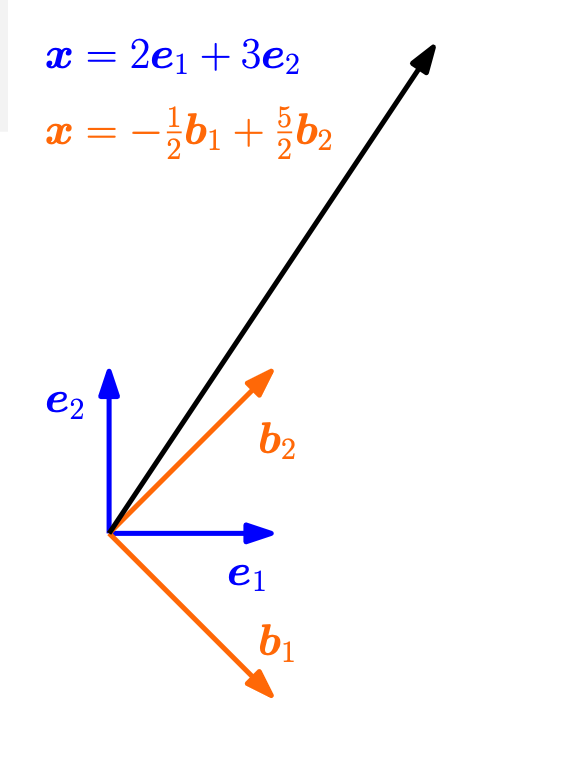
\includegraphics[width=0.5\textwidth,height=\textheight]{qmds/../images/coordinate.png}

}

\caption{기저의 변화에 대한 죄표의 변화}

\end{figure}%

이 예제에서 본 것처럼 기저가 변하면 동일한 원소에 대해서도 좌표가
달라진다.

만약 기저가 변했다면 좌표는 어떻게 변하는지를 알아야 한다. 이차원 공간의
임의의 벡터 \(\pmb x\) 에 대하여 두 기저 \(B\) 와 \(\tilde B\) 에 대하여
식~\ref{eq-coordi-ex1} 과 식~\ref{eq-coordi-ex2} 의 관계를 이용하면
다음과 같은 식을 얻을 수 있다.

\[
\begin{aligned}
& \quad \tilde {\pmb B}  \pmb \alpha_{\tilde B} = \pmb B \pmb \alpha_B  \\
\Rightarrow  & \quad  \pmb \alpha_{\tilde B}  = \tilde {\pmb B}^{-1} \pmb B  \pmb \alpha_B  \\
\Rightarrow &  \quad   \pmb \alpha_{\tilde B}  =\tilde {\pmb B}^{-1} \pmb I \pmb \alpha_B  \\
\Rightarrow &  \quad   \pmb \alpha_{\tilde B}  =\tilde {\pmb B}^{-1} \pmb \alpha_B  \\
\Rightarrow  & \quad   \pmb \alpha_{\tilde B}  = 
\begin{bmatrix}
1 & 1 \\
-1 & 1 
\end{bmatrix}^{-1}
\pmb \alpha_B  \\
\Rightarrow  & \quad \pmb \alpha_{\tilde B} =
\begin{bmatrix}
1/2 & -1/2 \\
1/2 & 1/2 
\end{bmatrix}
\pmb \alpha_B 
\end{aligned}
\] 따라서 기저가 변하면 좌표는 위와 같은 식으로 변한다.

\section{변환행렬}\label{uxbcc0uxd658uxd589uxb82c}

\subsection{정의}\label{uxc815uxc758}

이제 두 개의 벡터공간 \(V\) 와 \(W\) 에 대하여 선형사상 \(\Phi\) 가
정의되어 있고

\[ \Phi : V \rightarrow W \]

벡터공간 \(V\) 와 \(W\) 에 대한 기저가 각각
\(B=(\pmb b_1, \pmb b_2, \dots, \pmb b_n)\) 와
\(C = (\pmb c_1, \pmb c_2, \cdots, \pmb c_m)\) 이라고 하자.

이제 벡터공간 \(V\) 의 기저에 대한 선향사상의 원소가 벡터공간 \(W\) 의
기저로 다음과 같이 표현된다고 하자.

\begin{equation}\phantomsection\label{eq-coordi-trans1}{ 
\begin{aligned}
\Phi(\pmb b_1) &= a_{11} \pmb c_1 + a_{21} \pmb c_2 + \cdots + a_{m1} \pmb c_m \\
\Phi(\pmb b_2) &= a_{12} \pmb c_1 + a_{22} \pmb c_2 + \cdots + a_{m2} \pmb c_m \\
\cdots \\
\Phi(\pmb b_n) &= a_{1n} \pmb c_1 + a_{2n} \pmb c_2 + \cdots + a_{mn} \pmb c_m \\
\end{aligned}
}\end{equation}

식~\ref{eq-coordi-trans1} 에서 나타난 계수 \(a_{ij}\) 을
\(m \times n\)-행렬 \(\pmb A_{\Phi}\) 로 다음과 같이 표현할 수 있다.

\begin{equation}\phantomsection\label{eq-coordi-trans2}{
\pmb A_{\Phi} =
\begin{bmatrix}
a_{11} & a_{12} & \cdots & a_{1n} \\
a_{21} & a_{22} & \cdots & a_{2n} \\
\vdots & \vdots & \ddots & \vdots \\
a_{m1} & a_{m2} & \cdots & a_{mn} \\
\end{bmatrix}
}\end{equation}

식~\ref{eq-coordi-trans1} 에 나타난 행렬 \(\pmb A_{\Phi}\) 를
\textbf{변환행렬(transformation matrix)}이라고 부르며 이 변환행렬은 각
벡터공간의 기저 \(B\) 와 \(C\)에 따라 정의되는 것에 유의하자.

\subsection{좌표와
변환행렬}\label{uxc88cuxd45cuxc640-uxbcc0uxd658uxd589uxb82c}

만약 \(\hat {\pmb x}\) 가 벡터공간 \(V\) 에서 기저 \(B\) 에 대한 원소
\(\pmb x\)의 좌표이고

\[ \pmb x = \pmb B \hat {\pmb x} \]

\(\hat {\pmb y}\) 가 벡터공간 \(W\) 에서 기저 \(C\) 에 대한 선형사상
\(\pmb y = \Phi(\pmb x)\)의 좌표이면

\[ \pmb y = \pmb C \hat {\pmb y} \]

두 좌표 \(\hat {\pmb x}\) 와 \(\hat {\pmb y}\) 사이의 관계는 다음과
같다.

\begin{equation}\phantomsection\label{eq-coordi-trans3}{ \hat {\pmb y} = \pmb A_{\Phi} \hat {\pmb x} }\end{equation}

참고로 \(\RR^n\) 에서 \(\RR^m\) 으로의 선형사상
\(\Phi: \RR^n \rightarrow \RR^m\) 를 생각하고 각 공간의 기저를 표준
기저(standard basis)로 고려하면 변환행렬 \(\pmb A_{\Phi}\) 는 선형사상
\(\pmb y = \Phi(\pmb x )\) 을 나타내는 \(m \times n\) 행렬이다.

\begin{equation}\phantomsection\label{eq-coordi-trans4}{ \pmb y = \pmb A_{\Phi} \pmb x }\end{equation}

\subsection{예제}\label{uxc608uxc81c-1}

\begin{itemize}
\tightlist
\item
  부교재 Example 2.21 (Transformation Matrix) 참조
\item
  부교재 Example 2.22 (Linear Transformations of Vectors) 참조
\end{itemize}

\bookmarksetup{startatroot}

\chapter{기저변환과 변환행렬}\label{linear_transform_basis}

\begin{tcolorbox}[enhanced jigsaw, colback=white, colframe=quarto-callout-note-color-frame, opacityback=0, toprule=.15mm, leftrule=.75mm, titlerule=0mm, opacitybacktitle=0.6, title=\textcolor{quarto-callout-note-color}{\faInfo}\hspace{0.5em}{노트}, colbacktitle=quarto-callout-note-color!10!white, breakable, bottomrule=.15mm, bottomtitle=1mm, toptitle=1mm, arc=.35mm, left=2mm, rightrule=.15mm, coltitle=black]

강의 슬라이드 12번 기저변환과 변환행렬의 주제는 추후에 강의합니다.

\end{tcolorbox}

\bookmarksetup{startatroot}

\chapter{선형변환의 핵과 상}\label{linear_kernel}

\section{핵과 상의 정의}\label{uxd575uxacfc-uxc0c1uxc758-uxc815uxc758}

\begin{definition}[선형변환의 핵과
상]\protect\hypertarget{def-kernel}{}\label{def-kernel}

벡터공간 \(V\), \(W\) 사이의 선형사상 \(T :V \rightarrow W\)를 고려하자.
선형사상 \(T\) 의핵(kernel) \(Ker(T)\) 또는 영공간(null space)
\(N (T )\) 는 다음과 같이 정의된다:

\[ ker(T) = N (T ) = \{ \pmb v \in V \mid T( \pmb v) = \pmb 0 \} \]

또한 선형사상 \(T\) 의 상(range) 또는 치역(image) \(Im(T)\) 는 다음과
같이 정의된다:

\[ Im(T) = T(V) = \{ T(\pmb v) \mid \in V \} \]

\end{definition}

\begin{center}\rule{0.5\linewidth}{0.5pt}\end{center}

\begin{figure}[H]

{\centering 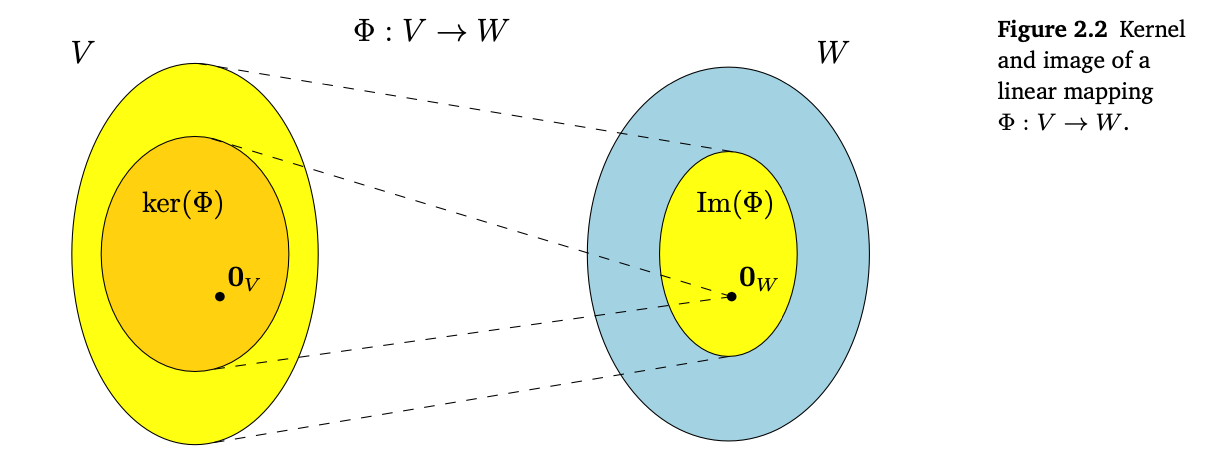
\includegraphics[width=0.8\textwidth,height=\textheight]{qmds/../images/linear_kernel.png}

}

\caption{선형변환의 핵과 상}

\end{figure}%

\begin{center}\rule{0.5\linewidth}{0.5pt}\end{center}

\subsection{예제}\label{uxc608uxc81c-2}

\begin{itemize}
\tightlist
\item
  부교재 Example 2.25 (Image and Kernel of a Linear Mapping)
\end{itemize}

\bookmarksetup{startatroot}

\chapter{아핀공간}\label{affine}

\begin{tcolorbox}[enhanced jigsaw, colback=white, colframe=quarto-callout-note-color-frame, opacityback=0, toprule=.15mm, leftrule=.75mm, titlerule=0mm, opacitybacktitle=0.6, title=\textcolor{quarto-callout-note-color}{\faInfo}\hspace{0.5em}{노트}, colbacktitle=quarto-callout-note-color!10!white, breakable, bottomrule=.15mm, bottomtitle=1mm, toptitle=1mm, arc=.35mm, left=2mm, rightrule=.15mm, coltitle=black]

강의 슬라이드 14번 아핀공간의 주제는 추후에 강의합니다.

\end{tcolorbox}

\bookmarksetup{startatroot}

\chapter{유클리드공간 위에서의 내적}\label{inner_product_1}

\begin{tcolorbox}[enhanced jigsaw, colback=white, colframe=quarto-callout-note-color-frame, opacityback=0, toprule=.15mm, leftrule=.75mm, titlerule=0mm, opacitybacktitle=0.6, title=\textcolor{quarto-callout-note-color}{\faInfo}\hspace{0.5em}{노트}, colbacktitle=quarto-callout-note-color!10!white, breakable, bottomrule=.15mm, bottomtitle=1mm, toptitle=1mm, arc=.35mm, left=2mm, rightrule=.15mm, coltitle=black]

\begin{itemize}
\tightlist
\item
  15번 슬라이드에서 코쉬-슈바르츠 부등식은 강의 범위가 아닙니다.
\item
  15번 슬라이드에서 삼각부등식(triangle inequality) 은 내용만 이해하고
  증명하지 않아도 됩니다.
\end{itemize}

\end{tcolorbox}

\section{중요한 내용과
정의}\label{uxc911uxc694uxd55c-uxb0b4uxc6a9uxacfc-uxc815uxc758-6}

\begin{itemize}
\tightlist
\item
  유클리드 공간에서 두 벡터의 내적(dot product, inner product)
\item
  내적의 성질
\end{itemize}

\bookmarksetup{startatroot}

\chapter{벡터공간 위에서의 내적}\label{inner_product_2}

\begin{tcolorbox}[enhanced jigsaw, colback=white, colframe=quarto-callout-note-color-frame, opacityback=0, toprule=.15mm, leftrule=.75mm, titlerule=0mm, opacitybacktitle=0.6, title=\textcolor{quarto-callout-note-color}{\faInfo}\hspace{0.5em}{노트}, colbacktitle=quarto-callout-note-color!10!white, breakable, bottomrule=.15mm, bottomtitle=1mm, toptitle=1mm, arc=.35mm, left=2mm, rightrule=.15mm, coltitle=black]

\begin{itemize}
\tightlist
\item
  16번 슬라이드에서 대각합을 이용한 행렬 내적의 예(슬라이드 2,3,4
  페이지)는 강의 범위가 아닙니다.
\item
  16번 슬라이드에서 유클리드공간에서 양정치행렬을 이용한 내적(슬라이드
  6페이지)에 대한 정리(Theorem) 은 강의 범위가 아닙니다.
\end{itemize}

\end{tcolorbox}

\section{중요한 내용과
정의}\label{uxc911uxc694uxd55c-uxb0b4uxc6a9uxacfc-uxc815uxc758-7}

\begin{itemize}
\tightlist
\item
  벡터공간에서 내적의 정의

  \begin{itemize}
  \tightlist
  \item
    슬라이드 15번에서 유클리드 공간에서 벡터의 내적 성질은 사실
    벡터공간에서 내적의 정의입니다.
  \end{itemize}
\item
  노름(Norm)의 정의와 성질
\item
  거리의 정의와 성질
\end{itemize}

\bookmarksetup{startatroot}

\chapter{직교기저}\label{ortho_normal_base}

\section{중요한 내용과
정의}\label{uxc911uxc694uxd55c-uxb0b4uxc6a9uxacfc-uxc815uxc758-8}

\begin{itemize}
\tightlist
\item
  직교의 정의
\item
  직교 기저의 정의와 성질
\item
  직교여공간의 정의
\end{itemize}

\bookmarksetup{startatroot}

\chapter{직선으로의 정사영}\label{projection_1}

\section{직선으로의
사영}\label{uxc9c1uxc120uxc73cuxb85cuxc758-uxc0acuxc601}

\begin{figure}

\centering{

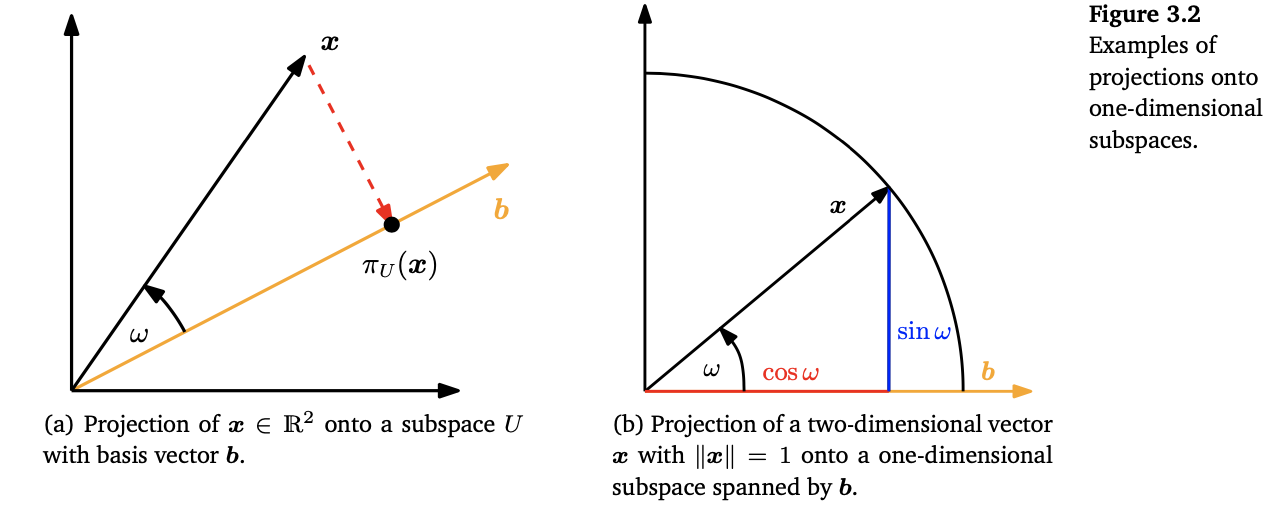
\includegraphics{qmds/../images/projection_line.png}

}

\caption{\label{fig-projection-line}직선으로의 사영}

\end{figure}%

\begin{enumerate}
\def\labelenumi{\arabic{enumi}.}
\tightlist
\item
  벡터 \(\pmb b\) 의 방향과 같은 벡터들 중에 벡터 \(\pmb x\) 와 가장
  가까운 벡터를 \(\pi_U(\pmb x)\) 라고 하자. 이 벡터는 \(\pmb x\) 에서
  직선 \(\pmb b\) 에 내린 사영(projection)이며 다음을 만족해야 한다.
\end{enumerate}

\begin{equation}\phantomsection\label{eq-projection-1}{
\left\langle\pmb{x}-\pi_U(\pmb{x}), \pmb{b}\right\rangle=0
}\end{equation}

\begin{enumerate}
\def\labelenumi{\arabic{enumi}.}
\setcounter{enumi}{1}
\tightlist
\item
  사영 \(\pi_U(\pmb x)\) 는 벡터 \(\pmb b\) 의 방향이므로 어떤 스칼라
  \(\lambda\) 가 존재하여 다음을 만족해야 한다.
\end{enumerate}

\[
\pi_U(\pmb{x})=\lambda \pmb{b}
\]

\begin{enumerate}
\def\labelenumi{\arabic{enumi}.}
\setcounter{enumi}{2}
\tightlist
\item
  식~\ref{eq-projection-1} 에서 제시된 직교하는 성질을 다시 쓰면 조건과
  같다.
\end{enumerate}

\[
\langle\pmb{x}-\lambda \pmb{b}, \pmb{b}\rangle=0 .
\]

\begin{enumerate}
\def\labelenumi{\arabic{enumi}.}
\setcounter{enumi}{3}
\tightlist
\item
  내적의 성질을 이용하면 다음을 얻을 수 있다. \[
  \langle\pmb{x}, \pmb{b}\rangle-\lambda\langle\pmb{b}, \pmb{b}\rangle=0 \Longleftrightarrow \lambda=\frac{\langle\pmb{x}, \pmb{b}\rangle}{\langle\pmb{b}, \pmb{b}\rangle}=\frac{\langle\pmb{b}, \pmb{x}\rangle}{\|\pmb{b}\|^2} .
  \] 따라서 스칼라 \(\lambda\) 는 다음과 같다.
\end{enumerate}

\[
\lambda=\frac{\pmb{b}^{\top} \pmb{x}}{\pmb{b}^{\top} \pmb{b}}=\frac{\pmb{b}^{\top} \pmb{x}}{\|\pmb{b}\|^2}
\]

\begin{enumerate}
\def\labelenumi{\arabic{enumi}.}
\setcounter{enumi}{4}
\tightlist
\item
  이제 벡터 \(\pmb b\) 의 방향으로의 벡터 \(\pmb x\)의 사영
  \(\pi_U(\pmb x)\) 는 다음과 같다.
\end{enumerate}

\begin{equation}\phantomsection\label{eq-projection-2}{
\pi_U(\pmb{x})=\lambda \pmb{b}=\frac{\langle\pmb{x}, \pmb{b}\rangle}{\|\pmb{b}\|^2} \pmb{b}=\frac{\pmb{b}^{\top} \pmb{x}}{\|\pmb{b}\|^2} \pmb{b}
}\end{equation}

\begin{enumerate}
\def\labelenumi{\arabic{enumi}.}
\setcounter{enumi}{5}
\tightlist
\item
  식~\ref{eq-projection-2} 에서 \(\pmb{b}^{\top} \pmb{x}\) 는
  스칼라이므로 다음과 같이 쓸 수 있으며 노름(norm)의 정의와 행렬의
  결합법칙을 이용하면 다음과 같다.
\end{enumerate}

\[ 
\begin{aligned}
\pi_U(\pmb{x}) &= \frac{\pmb{b}^{\top} \pmb{x}}{\|\pmb{b}\|^2} \pmb{b} \\
& = \pmb{b} \frac{\pmb{b}^{\top} \pmb{x}}{\|\pmb{b}\|^2} \quad (\text{스칼라 성질을 이용})\\
& =\frac{\pmb{b} (\pmb{b}^{\top} \pmb{x})}{\pmb{b}^{\top} \pmb{b}} \\ 
& =\frac{(\pmb{b} \pmb{b}^{\top}) \pmb{x}}{\pmb{b}^{\top} \pmb{b}}  \quad (\text{결합법칙을 이용})\\
& =\frac{\pmb{b} \pmb{b}^{\top}}{\pmb{b}^{\top} \pmb{b}} \pmb{x} \\
& =\frac{\pmb{b} \pmb{b}^{\top}}{\|\pmb{b}\|^2} \pmb{x} \\
& =\pmb P_{\pi}\pmb{x}
\end{aligned}
\]

\begin{enumerate}
\def\labelenumi{\arabic{enumi}.}
\setcounter{enumi}{6}
\tightlist
\item
  벡터 \(\pmb b\) 의 방향으로 사영행렬 \(\pmb P_{\pi}\) 는 다음과 같다.
\end{enumerate}

\begin{equation}\phantomsection\label{eq-projection-3}{
\pmb P_{\pi} = \frac{\pmb{b} \pmb{b}^{\top}}{\|\pmb{b}\|^2} 
}\end{equation}

식~\ref{eq-projection-3} 에서 \(\pmb{b} \pmb{b}^{\top}\) 는 정방행렬이고
\(\|\pmb{b}\|^2\)는 스칼라임에 유의하자.

\begin{tcolorbox}[enhanced jigsaw, colback=white, colframe=quarto-callout-important-color-frame, opacityback=0, toprule=.15mm, leftrule=.75mm, titlerule=0mm, opacitybacktitle=0.6, title=\textcolor{quarto-callout-important-color}{\faExclamation}\hspace{0.5em}{사영행렬의 성질}, colbacktitle=quarto-callout-important-color!10!white, breakable, bottomrule=.15mm, bottomtitle=1mm, toptitle=1mm, arc=.35mm, left=2mm, rightrule=.15mm, coltitle=black]

이미 사영된 \(\pi_U(\boldsymbol{x})\) 에 다시 사영행렬
\(\boldsymbol{P}_\pi\) 을 곱해도 아무런 변화가 없다. 이는 벡터
\(\pmb x\) 를 이미 벡터 \(\pmb b\) 의 방향으로 사영했기 때문에 다시
사영해도 변화가 없다는 것을 의미한다.

즉, \(\boldsymbol{P}_\pi \pi_U(\boldsymbol{x})=\pi_U(\boldsymbol{x})\)
이다. 사영행렬 \(\boldsymbol{P}_\pi\) 가 모든 벡터 \(\boldsymbol{x}\) 에
대해
\(\boldsymbol{P}_\pi^2 \boldsymbol{x}=\boldsymbol{P}_\pi \boldsymbol{x}\)
를 만족한다는 것을 의미한다.

\[ \boldsymbol{P}_\pi^2 = \boldsymbol{P}_\pi \]

\end{tcolorbox}

\section{중요한 내용과
정의}\label{uxc911uxc694uxd55c-uxb0b4uxc6a9uxacfc-uxc815uxc758-9}

\begin{itemize}
\tightlist
\item
  슬라이드 18번의 5페이지에 나온 사영행렬에 대한 예제
\item
  부교재 Example 3.10
\end{itemize}

\bookmarksetup{startatroot}

\chapter{행렬식과 대각합}\label{trace-det}

\begin{tcolorbox}[enhanced jigsaw, colback=white, colframe=quarto-callout-note-color-frame, opacityback=0, toprule=.15mm, leftrule=.75mm, titlerule=0mm, opacitybacktitle=0.6, title=\textcolor{quarto-callout-note-color}{\faInfo}\hspace{0.5em}{노트}, colbacktitle=quarto-callout-note-color!10!white, breakable, bottomrule=.15mm, bottomtitle=1mm, toptitle=1mm, arc=.35mm, left=2mm, rightrule=.15mm, coltitle=black]

이 노트의 내용은 부교재 100-105쪽의 내용을 요약한 것이다.

\end{tcolorbox}

\section{용어}\label{uxc6a9uxc5b4}

\begin{itemize}
\tightlist
\item
  determinant : 행렬식
\item
  trace : 대각합
\end{itemize}

\begin{tcolorbox}[enhanced jigsaw, colback=white, colframe=quarto-callout-caution-color-frame, opacityback=0, toprule=.15mm, leftrule=.75mm, titlerule=0mm, opacitybacktitle=0.6, title=\textcolor{quarto-callout-caution-color}{\faFire}\hspace{0.5em}{주의}, colbacktitle=quarto-callout-caution-color!10!white, breakable, bottomrule=.15mm, bottomtitle=1mm, toptitle=1mm, arc=.35mm, left=2mm, rightrule=.15mm, coltitle=black]

행렬식과 대각합은 정방행렬(square matrix)에 대해서만 정의된다.

\end{tcolorbox}

\section{행렬식}\label{uxd589uxb82cuxc2dd}

\#\#행렬식의 정의

정방행렬(square matrix) \(\pmb A\) 의 행렬식(determinant)는
\(\operatorname{det}(\pmb A)\) 로 표기한다.

\(A \in \mathbb{R}^{2 \times 2}\) 의 행렬식은 다음과 같이 계산한다.

\[
\operatorname{det}(\boldsymbol{A})=\left|\begin{array}{ll}
a_{11} & a_{12} \\
a_{21} & a_{22}
\end{array}\right|=a_{11} a_{22}-a_{12} a_{21} .
\]

\subsection{역행렬과 Rank}\label{uxc5eduxd589uxb82cuxacfc-rank}

\begin{itemize}
\tightlist
\item
  Theorm 4.1. 과 Theorem 4.3
\end{itemize}

행렬 \(\pmb A\) 가 \$n \times n \$ 정방행렬(square matrix) 인 경우 다음
3개의 문장이 동치(equivalent)임을 보여준다.

\begin{itemize}
\tightlist
\item
  \(\operatorname{det}(\boldsymbol{A}) \ne 0\)
\item
  \(rank(\boldsymbol{A}) = n\)
\item
  \(\boldsymbol{A}\)은 역행렬이 존재한다
\end{itemize}

\subsection{삼각행렬의
행렬식}\label{uxc0bcuxac01uxd589uxb82cuxc758-uxd589uxb82cuxc2dd}

행렬 \(\pmb T\) 가 상삼각행렬(upper triangular matrix) 또는
하삼각행렬(lower triangular matrix)이면 행렬식은 대각원소(diagonal
element)의 곱과 같다.

\[
\operatorname{det}(\boldsymbol{T}) = \prod_{i=1}^n T_{ii}
\]

\subsection{Laplace Expansion}\label{laplace-expansion}

\begin{itemize}
\tightlist
\item
  행렬식을 계산하는 방법 중 하나는 Laplace Expansion 이며 Theorem 4.2.
  에서 설명한다.
\item
  Example 4.3 꼭 읽어보기
\end{itemize}

\subsection{행렬식의 성질}\label{uxd589uxb82cuxc2dduxc758-uxc131uxc9c8}

\[ 
\operatorname{det}(\boldsymbol{A} \boldsymbol{B}) = \operatorname{det}(\boldsymbol{A}) \operatorname{det}(\boldsymbol{B})
\] \[ 
\operatorname{det}(\boldsymbol{A}^T) = \operatorname{det}(\boldsymbol{A})
\]

\[ 
\operatorname{det}(\boldsymbol{A}^{-1}) = \frac{1}{\operatorname{det}(\boldsymbol{A})}
\]

\[ 
\operatorname{det}(\lambda \boldsymbol{A}) = \lambda^n \operatorname{det}(\boldsymbol{A})
\]

\section{대각합}\label{uxb300uxac01uxd569}

대각합의 정의는 부교재 식 4.18 에서 정의된다.

\subsection{대각합의 성질}\label{uxb300uxac01uxd569uxc758-uxc131uxc9c8}

\begin{itemize}
\item
  \(\operatorname{tr}(\boldsymbol{A}+\boldsymbol{B})=\operatorname{tr}(\boldsymbol{A})+\operatorname{tr}(\boldsymbol{B})\)
  for \(\boldsymbol{A}, \boldsymbol{B} \in \mathbb{R}^{n \times n}\)
\item
  \(\operatorname{tr}(\alpha \boldsymbol{A})=\alpha \operatorname{tr}(\boldsymbol{A}), \alpha \in \mathbb{R}\)
  for \(\boldsymbol{A} \in \mathbb{R}^{n \times n}\)
\item
  \(\operatorname{tr}\left(\boldsymbol{I}_n\right)=n\)
\item
  \(\operatorname{tr}(\boldsymbol{A B})=\operatorname{tr}(\boldsymbol{B} \boldsymbol{A})\)
  for
  \(\boldsymbol{A} \in \mathbb{R}^{n \times k}, \boldsymbol{B} \in \mathbb{R}^{k \times n}\)
\end{itemize}

대각합은 교환법칙이 성립히기 떄문에 다음과 같은 성질이 성립한다.

\[
\operatorname{tr}(\boldsymbol{A} \boldsymbol{K} \boldsymbol{L})=\operatorname{tr}(\boldsymbol{K} \boldsymbol{L} \boldsymbol{A})
\] 벡터의 연산에서도 대각합의 교환법칙이 성립디어 다음과 같은 유용한
식이 성립한다.

\[
\operatorname{tr}\left(\boldsymbol{x} \boldsymbol{y}^{\top}\right)=\operatorname{tr}\left(\boldsymbol{y}^{\top} \boldsymbol{x}\right)=\boldsymbol{y}^{\top} \boldsymbol{x} \in \mathbb{R} .
\]

대각합의 교환법칙때문에 어떤 행렬의 앞에 특정 행렬을 곱하고, 뒤에
역행렬을 곱해도 대각합은 변하지 않는다.

\[
\operatorname{tr}\left(\boldsymbol{S}^{-1} \boldsymbol{A} \boldsymbol{S}\right) = \operatorname{tr}\left(\boldsymbol{A} \boldsymbol{S} \boldsymbol{S}^{-1}\right)=\operatorname{tr}(\boldsymbol{A})
\]

\section{특성다항식}\label{uxd2b9uxc131uxb2e4uxd56duxc2dd}

특성다항식(Characteristic polynomial)은 다음과 같이 정의된다 (부교재
definition 4.5)

실수 \(\lambda \in \mathbb{R}\) 와 정방행렬(square matrix)
\(\boldsymbol{A} \in \mathbb{R}^{n \times n}\) 에 대하여

\begin{equation}\phantomsection\label{eq-char-poly}{
\begin{aligned}
p_{\boldsymbol{A}}(\lambda) & :=\operatorname{det}(\boldsymbol{A}-\lambda \boldsymbol{I}) \\
& =c_0+c_1 \lambda+c_2 \lambda^2+\cdots+c_{n-1} \lambda^{n-1}+(-1)^n \lambda^n,
\end{aligned}
}\end{equation}

\subsection{행렬식과 대각합과의
관계}\label{uxd589uxb82cuxc2dduxacfc-uxb300uxac01uxd569uxacfcuxc758-uxad00uxacc4}

\[ c_0 = \operatorname{det}(\boldsymbol A)\]

\[ c_{n-1} = (-1)^n \operatorname{tr}(\boldsymbol A)\]

\bookmarksetup{startatroot}

\chapter{고유값과 고유벡터의 정의}\label{eigen-01}

\begin{tcolorbox}[enhanced jigsaw, colback=white, colframe=quarto-callout-note-color-frame, opacityback=0, toprule=.15mm, leftrule=.75mm, titlerule=0mm, opacitybacktitle=0.6, title=\textcolor{quarto-callout-note-color}{\faInfo}\hspace{0.5em}{노트}, colbacktitle=quarto-callout-note-color!10!white, breakable, bottomrule=.15mm, bottomtitle=1mm, toptitle=1mm, arc=.35mm, left=2mm, rightrule=.15mm, coltitle=black]

\begin{itemize}
\item
  이 노트의 내용은 부교재 105-110쪽의 내용을 요약한 것이다.
\item
  부교재 Example 4.5 반드시 공부하세요
\end{itemize}

\end{tcolorbox}

\section{용어}\label{uxc6a9uxc5b4-1}

\begin{itemize}
\tightlist
\item
  eigenvalue : 고유값
\item
  eigenvector : 고유벡터
\end{itemize}

\begin{tcolorbox}[enhanced jigsaw, colback=white, colframe=quarto-callout-caution-color-frame, opacityback=0, toprule=.15mm, leftrule=.75mm, titlerule=0mm, opacitybacktitle=0.6, title=\textcolor{quarto-callout-caution-color}{\faFire}\hspace{0.5em}{주의}, colbacktitle=quarto-callout-caution-color!10!white, breakable, bottomrule=.15mm, bottomtitle=1mm, toptitle=1mm, arc=.35mm, left=2mm, rightrule=.15mm, coltitle=black]

고유값과 고유벡터는 정방행렬(square matrix)에 대해서만 정의된다.

\end{tcolorbox}

\section{고유값과
고유벡터}\label{uxace0uxc720uxac12uxacfc-uxace0uxc720uxbca1uxd130}

\subsection{정의}\label{uxc815uxc758-1}

\(n\)-차원 정방행렬 \(\pmb A\) 이 있을 때, 다음 식을 만족하는
\(\lambda\) 와 벡터 \(\pmb x\)가 존재하면 \(\lambda\) 를 행렬 \(\pmb A\)
의 고유값(eigenvalue), \(\pmb x\) 를 행렬 \(\pmb A\) 의
고유벡터(eigenvector)라고 한다 (부교재 definition 4.6)

\[ \pmb A \pmb x = \lambda \pmb x \]

\begin{itemize}
\tightlist
\item
  고유벡터는 유일하지 않다. 즉, 벡터 \(\pmb x\) 가 고유벡터이면
  \(c \pmb x\) 도 고유벡터이다.
\end{itemize}

\[ \pmb A (c \pmb x) = c \pmb A \pmb x = c \lambda \pmb x = \lambda (c \pmb x) \]

\subsection{계산}\label{uxacc4uxc0b0}

다음 3개의 문장은 동치이다

\begin{itemize}
\tightlist
\item
  \(\lambda\) 는 행렬 \(\pmb A\) 의 고유값이다.
\item
  방정식 \((\pmb A - \lambda \pmb I)\pmb x = \pmb 0\) 은 영벡터이외의
  해를 가진다(nontrivial solution)
\item
  \(\lambda\) 는 행렬 \(\pmb A - \lambda \pmb I\) 의 행렬식이 0이다.
\end{itemize}

\begin{equation}\phantomsection\label{eq-char-poly2}{ \operatorname{det}(\pmb A - \lambda \pmb I) = 0 }\end{equation}

\begin{itemize}
\item
  \(\lambda\) 는 행렬 \(\pmb A - \lambda \pmb I\) 의 rank가 \(n\) 보다
  작다.
\item
  Theorem 4.8 에 의하면 위에서 행렬식이 0 인 방정식
  식~\ref{eq-char-poly2} 을 푸는 것은 식~\ref{eq-char-poly} 의 이 0 을
  푸는 것과 동일하다는 것이다.
\end{itemize}

\subsection{중복도와
고유공간}\label{uxc911uxbcf5uxb3c4uxc640-uxace0uxc720uxacf5uxac04}

부교재의 Definition 4.9, 4.10, 4.11 에 대한 내용입니다.

\begin{itemize}
\item
  대수적 중복도(algebraic multiplicity) 는 특성다항식
  식~\ref{eq-char-poly} 이 0인 방정식을 푸는 경우 다항식에서 고유값이
  중근(multiple root)의 해로 나타나는 차수를 의미한다.
\item
  기하적 중복도(geometric multiplicity) 는 고유값에 대응하는 고유벡터들
  중 선형독립인 고유벡터들의 최대 개수를 의미한다.
\item
  고유 공간(eigenspace)은 고유값에 대응하는 고유벡터들이 생성하는
  벡터공간을 의미한다.
\end{itemize}

\begin{center}\rule{0.5\linewidth}{0.5pt}\end{center}

\begin{exercise}[]\protect\hypertarget{exr-Example-20-1}{}\label{exr-Example-20-1}

3차원 행렬 \(\pmb A\) 가 다음과 같을 때

\[\pmb A=\left[\begin{array}{ccc}0 & 0 & -2 \\ 1 & 2 & 1 \\ 1 & 0 & 3\end{array}\right]\]

행렬 \(\pmb A\)의 특성다항식은 다음과 같다.

\[
\operatorname{det}(\lambda \pmb I -\pmb A)= 
\left|\begin{array}{ccc}
\lambda & 0 & 2 \\
-1 & \lambda-2 & -1 \\
-1 & 0 & \lambda-3
\end{array}\right|=(\lambda-1)(\lambda-2)^2
\] 참고로 특성방정식을 푸는 경우, 방정식
\(\operatorname{det}(\pmb A - \lambda \pmb I)=0\) 이나
\(\operatorname{det}(\lambda \pmb I -\pmb A)= 0\) 중 어느 것을 사용해도
상관없다.

첫번째 고유값은 \(\lambda_1=1\) 이다. 고유벡터를 구하기 위해서는 다음과
같은 방정식을 풀면 된다.

\[ (\lambda_1 \pmb I -\pmb A )\pmb x = \pmb 0  \]

위의 방정식을 풀면

\[
(\lambda_1 \pmb I -\pmb A )\pmb x= (\pmb I -\pmb A )\pmb x
=
\begin{bmatrix}
1 & 0 & 2 \\
-1 & -1 & -1 \\
-1 & 0 & -2
\end{bmatrix}
\begin{bmatrix}
x_1 \\
x_2 \\
x_3 \\
\end{bmatrix}
=
\begin{bmatrix}
0 \\
0 \\
0 \\
\end{bmatrix}
\]

아래와 같이 간단히 할 수 있으며

\[ x_1 = -2x_3, \quad x_2 = x_3 \] 다음과 같은 고유값과 고유벡터를 얻을
수 있다.

\[ \lambda_1=1 \quad \rightarrow \quad  x_1=\begin{bmatrix}-2 \\ 1 \\ 1\end{bmatrix} \]

\textbf{첫번째 고유값은 \(\lambda_1=1\) 이며 대수적 중복도는 1이고
기하적 중복도도 1이다.} 이 경우 고유공간 \(E_1\) 은 한 개의 고유벡터
\(\pmb x_1\) 이 생성하는 부분공간을 의미한다.

\[
E_1 = \text{span}\left\{\begin{bmatrix}-2 \\ 1 \\ 1\end{bmatrix} \right\}
\]

다음으로 두번째 고유값에 대한 방정식
\((\lambda_2 \pmb I -\pmb A )\pmb x = \pmb 0\) 을 풀면 다음과 같다.

\[
(\lambda_2 \pmb I -\pmb A )\pmb x= (2\pmb I -\pmb A )\pmb x =
\begin{bmatrix}
2 & 0 & 2 \\
-1 & 0 & -1 \\
-1 & 0 & -1
\end{bmatrix}
\begin{bmatrix}
x_1 \\
x_2 \\
x_3 \\
\end{bmatrix}
=
\begin{bmatrix}
0 \\
0 \\
0 \\
\end{bmatrix}
\]

이 방정식은 아래와 같이 간단히 할 수 있으며

\[ x_1 = -x_3 \] 다음과 같은 두 개의 고유벡터를 얻을 수 있다.

\[ 
\lambda_2=2\quad \rightarrow \quad  x_2=\begin{bmatrix}-1 \\ 0 \\ 1\end{bmatrix} 
\quad x_3=\begin{bmatrix}0 \\ 1 \\ 0\end{bmatrix} 
\]

위에서 \textbf{두번째 고유값은 \(\lambda_2=2\) 이며 대수적 중복도는
2이다.} 또한 \textbf{선형독립인 2개의 고유벡터를 구할 수 있으므로 기하적
중복도는 2이다.}

이 경우 \(E_2\) 는 두 개의 고유벡터 \(\pmb x_1, \pmb x_2\) 가 생성하는
부분공간을 의미한다.

\[
E_2 = \text{span}\left\{\begin{bmatrix}-1 \\ 0 \\ 1\end{bmatrix}, \begin{bmatrix}0 \\ 1 \\ 0\end{bmatrix}\right\}
\]

\(\blacksquare\)

\end{exercise}

\begin{center}\rule{0.5\linewidth}{0.5pt}\end{center}

이제 대수적 중복도와 기하적 중복도가 다른 경우에 대한 예제를 들어보자.

\begin{center}\rule{0.5\linewidth}{0.5pt}\end{center}

\begin{exercise}[]\protect\hypertarget{exr-Example-20-2}{}\label{exr-Example-20-2}

3차원 행렬 \(\pmb A\) 가 다음과 같을 때

\[\pmb A=\left[\begin{array}{ccc}1 & 0 & 2 \\ -1 & 1 & 3 \\ 0 & 0 & 2\end{array}\right]\]

행렬 \(\pmb A\)의 특성다항식은 다음과 같다.

\[
\operatorname{det}(\lambda \pmb I -\pmb A)= 
\left|\begin{array}{ccc}
\lambda-1 & 0 & -2 \\
1 & \lambda-1 & -3  \\
0 & 0 & \lambda-2
\end{array}\right|=(\lambda-1)^2(\lambda-2)
\] 첫번째 고유값은 \(\lambda_1=1\) 이다. 고유벡터를 구하기 위해서는
다음과 같은 방정식을 풀면 된다.

\[ (\lambda_1 \pmb I -\pmb A )\pmb x = \pmb 0  \]

위의 방정식을 풀면

\[
(\lambda_1 \pmb I -\pmb A )\pmb x= (\pmb I -\pmb A )\pmb x =
\begin{bmatrix}
0 & 0 & -2 \\
1 & 0 & -3 \\
0 & 0 & -1
\end{bmatrix}
\begin{bmatrix}
x_1 \\
x_2 \\
x_3 \\
\end{bmatrix}
=
\begin{bmatrix}
0 \\
0 \\
0 \\
\end{bmatrix}
\]

아래와 같이 간단히 할 수 있으며

\[ \quad x_1 = x_3 =0 \] 다음과 같은 하나의 고유벡터를 얻을 수 있다.

\[ \lambda_1=1 \quad \rightarrow \quad  x_1=\begin{bmatrix} 0 \\ 1 \\ 0 \end{bmatrix} \]

\textbf{첫번째 고유값은 \(\lambda_1=1\) 이며 대수적 중복도는 2이지만
기하적 중복도는 1이다.} 이 경우 고유공간 \(E_1\) 은 한 개의 고유벡터
\(\pmb x_1\) 이 생성하는 부분공간을 의미한다.

\[
E_1 = \text{span}\left\{\begin{bmatrix}0 \\ 1 \\ 0\end{bmatrix} \right\}
\]

다음으로 두번째 고유값에 대한 방정식
\((\lambda_2 \pmb I -\pmb A )\pmb x = \pmb 0\) 을 풀면 다음과 같다.

\[
(\lambda_2 \pmb I -\pmb A )\pmb x= (2\pmb I -\pmb A )\pmb x = 
\begin{bmatrix}
1 & 0 & 2 \\
1 & 1 & -3 \\
0 & 0 & 0
\end{bmatrix}
\begin{bmatrix}
x_1 \\
x_2 \\
x_3 \\
\end{bmatrix}
=
\begin{bmatrix}
0 \\
0 \\
0 \\
\end{bmatrix}
\]

이 방정식은 아래와 같이 간단히 할 수 있으며

\[ x_1 = -2x_3, \quad x_2=5x_3  \] 다음과 같은 한 개의 고유벡터를 얻을
수 있다.

\[ 
\lambda_2=2\quad \rightarrow \quad  x_2=\begin{bmatrix}-2 \\ 5 \\ 1\end{bmatrix} 
\]

위에서 \textbf{두번째 고유값은 \(\lambda_2=2\) 이며 대수적 중복도는
1이다.} 또한 \textbf{선형독립인 1개의 고유벡터를 구할 수 있으므로 기하적
중복도는 1이다.}

이 경우 \(E_2\) 는 한 개의 고유벡터 \(\pmb x_2\) 가 생성하는 부분공간을
의미한다.

\[
E_2 = \text{span}\left\{\begin{bmatrix}-2\\ 5 \\ 1\end{bmatrix}\right\}
\]

\(\blacksquare\)

\end{exercise}

\begin{center}\rule{0.5\linewidth}{0.5pt}\end{center}

\bookmarksetup{startatroot}

\chapter{고유값과 고유벡터의 성질}\label{eigen-02}

\begin{tcolorbox}[enhanced jigsaw, colback=white, colframe=quarto-callout-note-color-frame, opacityback=0, toprule=.15mm, leftrule=.75mm, titlerule=0mm, opacitybacktitle=0.6, title=\textcolor{quarto-callout-note-color}{\faInfo}\hspace{0.5em}{노트}, colbacktitle=quarto-callout-note-color!10!white, breakable, bottomrule=.15mm, bottomtitle=1mm, toptitle=1mm, arc=.35mm, left=2mm, rightrule=.15mm, coltitle=black]

이 노트의 내용은 부교재 110-119 쪽의 내용을 요약한 것이다.

\begin{itemize}
\item
  부교재 4.3 Cholesky Decomposition 은 시험범위에서 제외합니다.
\item
  부교재 Definition 4.13 의 defective matrix 는 시험범위에서 제외합니다.
\item
  부교재 4.4절은 모두 시험범위에 포함됩니다. 특히 Example 4.11 중요하니
  꼭 공부하세요
\end{itemize}

\end{tcolorbox}

\section{중요한 성질}\label{uxc911uxc694uxd55c-uxc131uxc9c8}

\begin{itemize}
\item
  행렬 \(\pmb A\) 와 그 전치(transpose) \({\pmb A}^T\) 는 동일한
  고유값을 가지나 고유벡터는 같지 않을 수 있다.
\item
  대칭이고 양정치 행렬(symmetrix positive definite)은 항상 양의 실수
  고유값을 갖는다.
\item
  행렬 \(\pmb A\) 의 고유값이 모두 다르면 고유벡터들은 선형독립이다.
\item
  부교재 Theorem 4.15, Example 4.8
\item
  부교재 Theorem 4.16, Theorem 4.17
\end{itemize}

\section{고유값 분해와
대각화}\label{uxace0uxc720uxac12-uxbd84uxd574uxc640-uxb300uxac01uxd654}

\begin{itemize}
\tightlist
\item
  고유값분해: Eigendecomposition
\item
  대각화 : Diagonalization
\end{itemize}

\bookmarksetup{startatroot}

\chapter{특이값 분해}\label{sdv-01}

\begin{tcolorbox}[enhanced jigsaw, colback=white, colframe=quarto-callout-note-color-frame, opacityback=0, toprule=.15mm, leftrule=.75mm, titlerule=0mm, opacitybacktitle=0.6, title=\textcolor{quarto-callout-note-color}{\faInfo}\hspace{0.5em}{노트}, colbacktitle=quarto-callout-note-color!10!white, breakable, bottomrule=.15mm, bottomtitle=1mm, toptitle=1mm, arc=.35mm, left=2mm, rightrule=.15mm, coltitle=black]

\begin{itemize}
\item
  시험 범위는 부교재 119-129 쪽입니다 (4.5절)
\item
  부교재 4.3 Example 4.13 중요하니 꼭 공부하세요
\item
  시험은 과제 3 번과 유사하게 출제됩니다.
\item
  4.6절은 시험범위에서 제외됩니다.
\end{itemize}

\end{tcolorbox}

\bookmarksetup{startatroot}

\chapter{벡터 미분}\label{vector-cal-01}

\begin{tcolorbox}[enhanced jigsaw, colback=white, colframe=quarto-callout-note-color-frame, opacityback=0, toprule=.15mm, leftrule=.75mm, titlerule=0mm, opacitybacktitle=0.6, title=\textcolor{quarto-callout-note-color}{\faInfo}\hspace{0.5em}{노트}, colbacktitle=quarto-callout-note-color!10!white, breakable, bottomrule=.15mm, bottomtitle=1mm, toptitle=1mm, arc=.35mm, left=2mm, rightrule=.15mm, coltitle=black]

\begin{itemize}
\tightlist
\item
  이 장은 부교재 139-159쪽에 대한 정리입니다.
\item
  5.4 Gradients of Matrices 는 시험범위에 포함되지 않습니다.
\end{itemize}

\end{tcolorbox}

\section{용어}\label{uxc6a9uxc5b4-2}

\begin{itemize}
\tightlist
\item
  vector differential: 벡터 미분
\item
  partial derivative: 편미분
\item
  gradient: 그레디언트
\item
  Jacobian: 야코비안, 자코비안
\end{itemize}

\section{벡터 미분의
표기법}\label{uxbca1uxd130-uxbbf8uxbd84uxc758-uxd45cuxae30uxbc95}

이제 다변량함수(multivariate function), \(f: \RR^n \rightarrow \RR^m\)에
대한 미분을 생각해보자.

먼저 간단한 예제를 고려해 보자. 두 열벡터
\(\pmb x=(x_1,x_2)^t \in \RR_2\), \(\pmb y=(y_1,y_2,y_3)^t \in \RR^3\)를
고려하고 다음과 같은 함수로 두 벡터의 관계가 정의된다고 하자.

\begin{equation}\phantomsection\label{eq-vec-cal-xy}{ 
y_1 = x_1^2 + x_2, \quad y_2= \exp (x_1) + 3 x_2, \quad y_3 = \sin(x_1) + x_2^3 
}\end{equation}

위의 관계를 함수 관계 \(\pmb f: \RR^2 \rightarrow \RR^3\) 로 나타내보면

\[ 
 \pmb f(\pmb x) = 
\begin{bmatrix} f_1(\pmb x) \\ f_2 (\pmb x) \\ f_3(\pmb x) \end{bmatrix} = 
\begin{bmatrix} x_1^2 + x_2 \\ \exp (x_1) + 3 x_2 \\ \sin(x_1) + x_2^3 \end{bmatrix} 
\]

이러한 경우 다변량 함수 \(\pmb f\)를 벡터 \(\pmb x\)로 미분하려면, 즉
미분 표기법을 이용하려면 편미분을 한 결과를 행렬의 형태를 정해야한다.

\[  \pardifftwo{ \pmb f}{\pmb x} = (n \times m)-\text{matrix} \quad \text{ or }  \quad (m \times n)-\text{matrix}? \]

일단 각각의 편미분 \(\pardifftwo{f_i}{x_j}\)를 구해야 하며 이는 scalar
미분으로 쉽게 구해진다.

\begin{equation}\phantomsection\label{eq-par_deriv}{
\begin{aligned}
\pardifftwo{  f_1}{ x_1} & = 2x_1, & \quad \pardifftwo{  f_2}{ x_1} & = \exp(x_1), & \quad
\pardifftwo{  f_3}{ x_1} & = \cos(x_1) \\
\pardifftwo{  f_1}{ x_2} & = 1,    & \quad \pardifftwo{  f_2}{ x_1} & = 3,         & \quad
\pardifftwo{  f_3}{ x_1} & = 3 x_2^2 \\
\end{aligned}
}\end{equation}

이제 이제 편미분값들을 행렬의 형태로 정리해보자. 편미분을 행렬에 배치할
떄 다음과 같은 규칙을 사용할 것이다.

\begin{itemize}
\tightlist
\item
  행렬의 행은 \(\pmb f\)의 차원 \(m\) 과 같다.
\item
  행렬의 열은 \(\pmb x\)의 차원 \(n\) 과 같다.
\end{itemize}

위와 같이 편미분을 배치하는 벡타 미분 표기법을 분자 표기법 (Numerator
layout)이라고 한다.

\begin{tcolorbox}[enhanced jigsaw, colback=white, colframe=quarto-callout-note-color-frame, opacityback=0, toprule=.15mm, leftrule=.75mm, titlerule=0mm, opacitybacktitle=0.6, title=\textcolor{quarto-callout-note-color}{\faInfo}\hspace{0.5em}{분자 표기법 (Numerator layout)}, colbacktitle=quarto-callout-note-color!10!white, breakable, bottomrule=.15mm, bottomtitle=1mm, toptitle=1mm, arc=.35mm, left=2mm, rightrule=.15mm, coltitle=black]

\[ 
\pmb J = \nabla_x \pmb x =\pardifftwo{ \pmb f}{\pmb x}  \equiv \pardifftwo{ \pmb f}{\pmb x^t}
\underset{def}{\equiv} \begin{bmatrix}
\pardifftwo{  f_1}{ x_1} &  \pardifftwo{  f_1}{ x_2}  \\
\pardifftwo{  f_2}{ x_1} &  \pardifftwo{  f_2}{ x_2}  \\
\pardifftwo{  f_3}{ x_1} &  \pardifftwo{  f_3}{ x_2}
\end{bmatrix}
=  \begin{bmatrix}
2x_1 &  1  \\
\exp(x_1) &  3  \\
\cos(x_1) &  3x_2^2
\end{bmatrix}
\] \(\pmb J\)는 야코비안 행렬(Jacobian matrix)이라고 부른다.

\end{tcolorbox}

이제 이러한 분자표기법의 특별한 결과를 알아보자

\begin{itemize}
\item
  \(f: \RR^n \rightarrow \RR^1\) 인 경우

  \(f: \RR^n \rightarrow \RR^1\) 인 경우 벡터미분 결과를
  \textbf{그레디언트(gradient)}라고 부르며 다음과 같이 표기된다.
\end{itemize}

\[ 
\nabla_x f = \pardifftwo{ f}{\pmb x} = 
\begin{bmatrix} \pardifftwo{ f}{x_1} & \pardifftwo{ f}{x_2} & \cdots & \pardifftwo{ f}{x_n} \end{bmatrix} 
\]

\begin{itemize}
\tightlist
\item
  \(f: \RR^1 \rightarrow \RR^m\) 인 경우
\end{itemize}

\[ 
\pardifftwo{\pmb f}{x} = 
\begin{bmatrix} 
\pardifftwo{ f_1}{x} \\
\pardifftwo{ f_2}{x} \\
\vdots \\
\pardifftwo{ f_m}{x} 
\end{bmatrix} 
\]

참고로 식~\ref{eq-vec-cal-xy} 에서 정의한 함수 관계를 두 벡터 \(\pmb x\)
와 \pmb y\$ 의 사상관계로 보면

\[ \pmb f : \pmb x \mapsto \pmb y \] 다음과 같이 그레디언트 벡터를
표기할 수 있다.

\[  \pardifftwo{ \pmb f}{\pmb x} = \pardifftwo{ \pmb y}{\pmb x}
=
\begin{bmatrix}
\pardifftwo{  y_1}{ x_1} &  \pardifftwo{  y_1}{ x_2}  \\
\pardifftwo{  y_2}{ x_1} &  \pardifftwo{  y_2}{ x_2}  \\
\pardifftwo{  y_3}{ x_1} &  \pardifftwo{  y_3}{ x_2}
\end{bmatrix}
\]

\section{함성함수의
미분법}\label{uxd568uxc131uxd568uxc218uxc758-uxbbf8uxbd84uxbc95}

이제 합성함수의 미분법(chain rule)에 대하여 알아보자.

두 개의 함수

\[
\pmb g :\RR^n \mapsto \RR^m, \quad \pmb f :\RR^m \mapsto \RR^p
\] 가 있을 때, \(\pmb f\)와 \(\pmb g\)의 합성함수 \(\pmb h\)는 다음과
같이 정의된다.

\[ \pmb h( \pmb x) = \pmb f( \pmb g( \pmb x)) = \pmb f \circ \pmb g\]
즉,

\[ 
\pmb h : \RR^n \mapsto \RR^m \mapsto \RR^p
\]

이러한 합성함수의 미분은 다음과 같이 계산된다.

\begin{equation}\phantomsection\label{eq-vec-chain-01}{
\pardifftwo{ \pmb h}{\pmb x} = \pardifftwo{ \pmb f \circ \pmb g}{\pmb x} = \pardifftwo{ \pmb f}{\pmb g} \pardifftwo{ \pmb g}{\pmb x}
}\end{equation}

식~\ref{eq-vec-chain-01} 에서 \(\pardifftwo{ \pmb f}{\pmb g}\)는
\(p \times m\) Jacovian 벡터이고

\[ 
\pardifftwo{ \pmb f}{\pmb g} 
\begin{bmatrix}
\pardifftwo{  f_1}{ g_1} &  \pardifftwo{  f_1}{ g_2} & \cdots &  \pardifftwo{  f_1}{ g_m} \\
\pardifftwo{  f_2}{ g_1} &  \pardifftwo{  f_2}{ g_2} & \cdots &  \pardifftwo{  f_2}{ g_m} \\
\vdots & \vdots & \ddots & \vdots \\
\pardifftwo{  f_p}{ g_1} &  \pardifftwo{  f_p}{ g_2} & \cdots &  \pardifftwo{  f_p}{ g_m} \\
\end{bmatrix}
=(p \times m)
\]

\(\pardifftwo{ \pmb g}{\pmb x}\)는 \(n \times m\) Jacovian 벡터이다

\[
\pardifftwo{ \pmb g}{\pmb x} =
\begin{bmatrix}
\pardifftwo{  g_1}{ x_1} &  \pardifftwo{  g_1}{ x_2} & \cdots &  \pardifftwo{  g_1}{ x_n} \\
\pardifftwo{  g_2}{ x_1} &  \pardifftwo{  g_2}{ x_2} & \cdots &  \pardifftwo{  g_2}{ x_n} \\
\vdots & \vdots & \ddots & \vdots \\
\pardifftwo{  g_m}{ x_1} &  \pardifftwo{  g_m}{ x_2} & \cdots &  \pardifftwo{  g_m}{ x_n} \\
\end{bmatrix}
= (n \times m)
\]

함성함수의 미분 공식을 차원으로 나타내면 다음과 같다.

\[
\underset{ p \times n} {\pardifftwo{ \pmb h}{\pmb x}} = \underset{ p \times m} {\pardifftwo{ \pmb f}{\pmb g}} \underset{ m \times n} {\pardifftwo{ \pmb g}{\pmb x}}
\]

\section{두 벡터 내적의
미분}\label{uxb450-uxbca1uxd130-uxb0b4uxc801uxc758-uxbbf8uxbd84}

\subsection{상수벡터와 변수벡터의
내적}\label{uxc0c1uxc218uxbca1uxd130uxc640-uxbcc0uxc218uxbca1uxd130uxc758-uxb0b4uxc801}

먼저 상수 벡터 \(\pmb a\)와 변수 벡터 \(\pmb x\)의 내적의 미분을 생각해
보자.

참고로 다음과 같이 두 벡터의 내적은 스칼라이다.

\[ \pmb a^T \pmb x = \pmb x^T \pmb a = a_1 x_1 + a_2x_2 + \dots + a_n x_n \]

따라서 그레이디언트를 구하는 방법과 같이 결과는 행백터로 표기된다.

\[
\pardifftwo{ \pmb a^T \pmb x}{\pmb x} = \pardifftwo{ \pmb x^T \pmb a}{\pmb x} = \pmb a^T =[a_1, a_2, \dots, a_n]
\]

위의 식에서 상수벡터 \(\pmb a\)는 가 전치로 앞에 나타나는 표현
\(\pmb a^T \pmb x\) 를 사용하면 결과 벡터 \(\pmb a^T\)가 행벡터로 그대로
나타나지므로 \textbf{내적의 미분 표기}로 사용할 것이다.

\begin{equation}\phantomsection\label{eq-vec-diff}{ 
\pardifftwo{ \pmb a^T \pmb x}{\pmb x} = \pmb a^T \pardifftwo{  \pmb x}{\pmb x} =\pmb a^T 
}\end{equation}

\subsection{상수벡터와 함수벡터의
내적}\label{uxc0c1uxc218uxbca1uxd130uxc640-uxd568uxc218uxbca1uxd130uxc758-uxb0b4uxc801}

더 나아가서 상수 벡터 \(\pmb a\)와 함수 벡터 \(\pmb f\)의 내적의 미분도
식~\ref{eq-vec-diff} 을 표시하는 동일한 논리로 다음과 같이 표기할 수
있다.

\begin{equation}\phantomsection\label{eq-vec-diff-0}{ 
\pardifftwo{ \pmb a^T \pmb f}{\pmb x} = \pmb a^T \pardifftwo{  \pmb f}{\pmb x}
}\end{equation}

참고로 식~\ref{eq-vec-diff-0} 에서 \(\pardifftwo{ \pmb f}{\pmb x}\)는
행벡터가 아닌 행렬로 나타날 수 있다.

\subsection{함수벡터와 함수벡터의
내적}\label{uxd568uxc218uxbca1uxd130uxc640-uxd568uxc218uxbca1uxd130uxc758-uxb0b4uxc801}

이제 다음과 같이 같은 공간으로 사상되는 두 함수 \(\pmb f\) 와 \(\pmb g\)
의 내적을 생각해 보자.

\[ \pmb f : \RR^n \mapsto \RR^m, \quad \pmb g : \RR^n \mapsto \RR^m\] 두
함수의 내적을 미분하는 경우 곱셉 법칙을 적용하여야 하는데 행렬의
곱셉에서는 교환법칙이 성립되지 않으므로 순서에 주의해야 한다.

내적 \(\pmb f^T \pmb g\) 를 각각 따로 미분해야 하는데 각 벡터에 대해
따로 미분을 실행해 보자

\begin{itemize}
\tightlist
\item
  \(\pmb f\) 를 미분하는 경우 \(\pmb g\) 는 상수 벡터 \(\pmb a\) 로
  취급한다. 그리고 식~\ref{eq-vec-diff-0} 를 적용한다.
\end{itemize}

\begin{equation}\phantomsection\label{eq-vec-diff-1}{
\pardifftwo{ \pmb f^T \pmb g}{\pmb x} = \pardifftwo{ \pmb f^T \pmb a}{\pmb x} = 
\pardifftwo{ \pmb a^T \pmb f}{\pmb x} = \pmb a^T \pardifftwo{ \pmb f}{\pmb x} =
\pmb g^T \pardifftwo{ \pmb f}{\pmb x} 
}\end{equation}

\begin{itemize}
\tightlist
\item
  \(\pmb g\) 를 미분하는 경우 \(\pmb f\) 는 상수 벡터 \(\pmb a\) 로
  취급한다. 그리고 식~\ref{eq-vec-diff-0} 를 적용한다.
\end{itemize}

\begin{equation}\phantomsection\label{eq-vec-diff-2}{
\pardifftwo{ \pmb f^T \pmb g}{\pmb x} = \pardifftwo{ \pmb a^T \pmb g}{\pmb x} = 
 \pmb a^T \pardifftwo{ \pmb g}{\pmb x} =
\pmb f^T \pardifftwo{ \pmb f}{\pmb x} 
}\end{equation}

이제 위의 두 결과 식~\ref{eq-vec-diff-1} 과 식~\ref{eq-vec-diff-2} 를
합치면 다음과 같은 최종적인 결과를 얻을 수 있다.

\begin{equation}\phantomsection\label{eq-vec-diff-prod}{
\pardifftwo{ \pmb f^T \pmb g}{\pmb x} = \pmb g^T \pardifftwo{ \pmb f}{\pmb x} + \pmb f^T \pardifftwo{ \pmb g}{\pmb x} 
}\end{equation}

\section{벡터 미분의
응용}\label{uxbca1uxd130-uxbbf8uxbd84uxc758-uxc751uxc6a9}

\subsection{선형사상의
미분상}\label{uxc120uxd615uxc0acuxc0c1uxc758-uxbbf8uxbd84uxc0c1}

이제 앞에서 배운 벡터의 미분을 이용하여 유용한 응용 공식을 유도해보자.

먼저 선형변환 \(\pmb y = \pmb A \pmb x\) 를 생각해 보자. 이때 (M
\times N)-\(\pmb A\)는 상수 행렬이다. 이때 \(\pmb y\)를 \(\pmb x\)로
미분하면 다음과 같다.

먼저 행렬 \(\pmb A\)의 \(i\) 번째 행을 \(\pmb a_i^T\)라고 하면

\[
\pmb A = \begin{bmatrix}
A_{11} & A_{12} & \dots & A_{1N} \\
A_{21} & A_{22} & \dots & A_{2N} \\
\vdots & \vdots & \ddots & \vdots \\
A_{M1} & A_{M2} & \dots & A_{MN} \\
\end{bmatrix}=
\begin{bmatrix}
\pmb a_1^T  \\
\pmb a_2^T  \\
\vdots \\
\pmb a_M^T  \\
\end{bmatrix}
\]

선형변환 \(\pmb f(\pmb x) = \pmb A \pmb x\) 로 정의하면 다음과 같이
나타낼 수 있다.

\[
\pmb A \pmb x=
\begin{bmatrix}
\pmb a_1^T \pmb x \\
\pmb a_2^T \pmb x \\
\vdots \\
\pmb a_M^T \pmb x \\
\end{bmatrix} =
\begin{bmatrix}
f_1(\pmb x) \\
f_2(\pmb x) \\
\vdots \\
f_M(\pmb x) \\
\end{bmatrix} 
= \pmb f(\pmb x) 
\]

따라서

\[
\pardifftwo{\pmb A \pmb x}{\pmb x}   = \pardifftwo{\pmb f (\pmb x)}{\pmb x} =
\begin{bmatrix}
\pardifftwo{f_1}{x_1} & \pardifftwo{f_1}{x_2} & \dots & \pardifftwo{f_1}{x_N} \\
\pardifftwo{f_2}{x_1} & \pardifftwo{f_2}{x_2} & \dots & \pardifftwo{f_2}{x_N} \\
\vdots & \vdots & \ddots & \vdots \\
\pardifftwo{f_M}{x_1} & \pardifftwo{f_M}{x_2} & \dots & \pardifftwo{f_M}{x_N} \\
\end{bmatrix} =
\begin{bmatrix}
A_{11} & A_{12} & \dots & A_{1N} \\
A_{21} & A_{22} & \dots & A_{2N} \\
\vdots & \vdots & \ddots & \vdots \\
A_{M1} & A_{M2} & \dots & A_{MN} \\
\end{bmatrix} = \pmb A
\] 따라서 선형사상의 미분은 그 자신이다.

\begin{equation}\phantomsection\label{eq-vec-diff-linear}{ \pardifftwo{\pmb A \pmb x}{\pmb x}  = \pmb A }\end{equation}

\subsection{이차형식의
미분}\label{uxc774uxcc28uxd615uxc2dduxc758-uxbbf8uxbd84}

이차형식 \(f(\pmb x) = \pmb x^T \pmb B \pmb x\) 을 미분하는 경우
식~\ref{eq-vec-diff-prod} 을 적용한다. 이 경우 \(\pmb f= \pmb x^T\) 이고
\(\pmb g = \pmb B \pmb x\) 이라고 놓고 식~\ref{eq-vec-diff-prod} 을
적용하면 다음과 같다.

\[
\begin{aligned}
\pardifftwo{\pmb x^T \pmb B \pmb x}{\pmb x} & = 
\pardifftwo{\pmb x^T (\pmb B \pmb x)}{\pmb x} \\
& =  (\pmb B \pmb x)^T \pardifftwo{ \pmb x}{\pmb x}  + 
\pmb x^T \pardifftwo{ (\pmb B \pmb x)}{\pmb x} \\
& =  \pmb x^T \pmb B^T  +  \pmb x^T \pmb B \\
& = \pmb x^T (\pmb B^T + \pmb B)
\end{aligned}
\]

만약 행렬 \(\pmb B\)가 대칭행렬이면 \(\pmb B^T = \pmb B\) 이므로 다음과
같이 간단하게 나타낼 수 있다.

\begin{equation}\phantomsection\label{eq-vec-diff-quad}{
\pardifftwo{\pmb x^T \pmb B \pmb x}{\pmb x} = \pmb x^T (\pmb B + \pmb B) = 2 \pmb x^T \pmb B
}\end{equation}

\subsection{최소제곱법의
미분}\label{uxcd5cuxc18cuxc81cuxacf1uxbc95uxc758-uxbbf8uxbd84}

부교재 Example 5.11 의 내용을 다음과 같이 정리할 수 있다.

\[ \pmb y = \pmb \Phi \pmb \theta, \quad\]

여기서 \(\boldsymbol{\theta} \in \mathbb{R}^D\) 는 모수벡터(parameter
vector), \(\boldsymbol{\Phi} \in \mathbb{R}^{N \times D}\) are
입력변수(input features), \(\boldsymbol{y} \in \mathbb{R}^N\) are the
관측값 벡터(observation vector).

다음으로 손실함수(loss function) \(L\) 과 오타벡터 \$\pmb \$ 를 다음과
같이 정의하자

\[
\begin{aligned}
& L(\boldsymbol{e}):=\|\boldsymbol{e}\|^2 = \pmb e^T \pmb e\\
& \boldsymbol{e}(\boldsymbol{\theta}):=\boldsymbol{y}-\boldsymbol{\Phi} \boldsymbol{\theta} .
\end{aligned}
\]

이때 손실함수 \(L\) 을 최소화하는 \(\boldsymbol{\theta}\) 를 구하는
문제는 손실함수 \(L\) 을 \(\boldsymbol{\theta}\) 로 미분하여 0 이 되는
\(\boldsymbol{\theta}\) 를 구하는 문제로 바뀐다.

이러한 경우 손실함수 \(L\) 을 \(\boldsymbol{\theta}\) 로 미분하는 경우
다음과 같이 정리할 수 있다.

\[
\begin{aligned}
\pardifftwo{L}{\pmb \theta} & =   \pardifftwo{L}{\pmb e} \pardifftwo{\pmb e}{\pmb \theta} \\
& =  \pardifftwo{\pmb e^T \pmb e}{\pmb e} \pardifftwo{(\pmb y - \pmb \Phi \pmb \theta)}{\pmb \theta} \\
& = 2\pmb e^T \pardifftwo {\pmb \Phi \pmb \theta}{\pmb \theta} \\
& = 2\pmb e^T \pmb \Phi \\
& = 2(\boldsymbol{y}-\boldsymbol{\Phi} \boldsymbol{\theta} ) ^T \pmb \Phi \\
\end{aligned}
\] 참고로 위의 식에서 첫 번째 식은 합성함수의
공식(식~\ref{eq-vec-chain-01}), 세 번째 식은 이차형식의
미분(식~\ref{eq-vec-diff-quad}) 과 선형사상의
미분(식~\ref{eq-vec-diff-linear}) 을 적용하였다.

\bookmarksetup{startatroot}

\chapter*{References}\label{references}
\addcontentsline{toc}{chapter}{References}

\markboth{References}{References}

\phantomsection\label{refs}
\begin{CSLReferences}{1}{0}
\bibitem[\citeproctext]{ref-math2020ml}
Deisenroth, Marc Peter, A Aldo Faisal, 와/과 Cheng Soon Ong. 2020.
\emph{Mathematics for machine learning}. Cambridge University Press.

\end{CSLReferences}


\backmatter

\end{document}
